\documentclass{article}
\usepackage{graphicx} % Required for inserting images
\usepackage{amsmath, amssymb}
\usepackage{tikz}
\usepackage{enumitem}
\usepackage{pdfpages}
\usepackage{subcaption}
\usepackage{booktabs,makecell,multirow}
\usepackage{float}
\usepackage[margin=0.75in]{geometry}
\usepackage[most]{tcolorbox}
\usepackage{siunitx}
\usepackage{hyperref}
\hypersetup{
  colorlinks=true,
  linkcolor=black,
  citecolor=black,
  urlcolor=blue
}
\geometry{margin=1in}

% ---------- SECTION STYLE ----------
\usepackage{titlesec}
\titleformat{\section}{\large\bfseries}{\thesection}{0.5em}{}[{\titlerule[0.4pt]}]
\titleformat{\subsection}{\normalsize\bfseries}{\thesubsection}{0.5em}{}

\tcbuselibrary{skins}
\tcbset{
  ansbox/.style={
    enhanced,
    colback=white,
    colframe=black,
    boxrule=0.7pt,
    arc=3pt,
    left=8pt, right=8pt, top=5pt, bottom=5pt
  }
}

% Code + boxes
\usepackage{tcolorbox}
\tcbuselibrary{breakable, skins}
\usepackage{fancyvrb}
\usepackage{minted}

\newtcolorbox{graybox}{
    colback=gray!10,
    colframe=gray!60,
    boxrule=0.6pt,
    arc=2mm,
    left=2mm,
    right=2mm,
    top=1mm,
    bottom=1mm
}

\newtcolorbox{assumptionbox}[1]{
    colback=gray!10,
    colframe=gray!70,
    title=#1,
    fonttitle=\bfseries,
    boxrule=0.6pt,
    arc=2mm,
    left=2mm,
    right=2mm,
    top=1mm,
    bottom=1mm
}

\begin{document}

\begin{titlepage}
	\centering
	
\includegraphics[width=0.5\textwidth]{Berkeleylogo.png}\par\vspace{2cm} 
	{\scshape\LARGE University of California Berkeley Haas School of Business \par} 
	\vspace{2cm}
	{\scshape\Large 230X: High Frequency Finance\par} 
	\vspace{0.8cm}
	{\huge\bfseries Final Assignment \par} 
	\vspace{1cm}
 
    {\Large\itshape Daisy Niu}\par 
    \texttt{daisy\_niu@berkeley.edu}\par 
	\vspace{0.5cm}
    {\Large\itshape Hrafnhildur Jonsdottir}\par 
    \texttt{hrafnhildur.jonsd@berkeley.edu}\par 
	\vspace{0.5cm}
    {\Large\itshape Paraj Goyal}\par 
    \texttt{paraj\_goyal@berkeley.edu}\par 
	\vspace{0.5cm}
    {\Large\itshape Reza Zamani}\par 
    \texttt{rezazamani@berkeley.edu}\par 
	\vspace{0.5cm}
    {\Large\itshape Saurabh Baranwal}\par 
    \texttt{saurabh\_baranwal@berkeley.edu}\par 
	\vspace{0.5cm}
    
        \vfill
        
	Fall 2026\par 
	Professor Terry Hendershott \& Dmitry Livdan \\
    GSI: Vinicio De Sola \& Soobin Kim\\ 
	\vfill

 % Bottom of the page
 {\large October 11, 2026\par}
\end{titlepage}


\section{Speed}

\subsection{Introduction}

In this assignment we study the Scholtus and van Dijk (2012) paper which looks into how much execution speed matters for simple technical trading rules. They apply 27,424 rules from seven rule families to three liquid ETFs (SPY, QQQQ and IWM) on NASDAQ from January to September 2009, and compare the return of each rule when it is executed instantly with its return when execution is delayed by 10 milliseconds up to 1 second. Their main finding is that delay hurts strategies that are profitable without delay. The loss becomes significant at 200 ms, and already at 50 ms on low volatility days. Strategies that lose money are not affected, which the authors attribute to competition for good signals. The economic size of the effect is small, but it grows over their sample period.\\

\noindent In this assignment we repeat the exercise on a smaller scale and on more recent data. We use three assets that differ in liquidity and market structure. The assets that were chosen are Nvidia (NVDA) as a highly liquid stock, Qorvo (QRVO) as a less liquid stock, and EUR/USD as the FX rate. Our sample is March 2025. We test two signals from the paper, Moving Average (MA) and Support and Resistance (SR), and add Order Flow Imbalance (OFI) as our own signal. Each signal is run on \$1,000,000 with execution delays of 0 ms, 100 ms and 1 second, and we measure the cost of delay as the drop in return relative to instant execution. We then relate that cost to how often prices change in each asset.

\subsection{Data and Methodology}

All data used in this assignment comes from Databento at the top of book level (MBP-1), which records every change to the best bid and ask together with all trades. For NVDA and QRVO we use the NASDAQ TotalView-ITCH feed, the same feed as used in the paper. For EUR/USD we use the front CME Euro FX future (6E) from the CME Globex feed, since FX has no single consolidated exchange. The sample covers the 21 trading days from March 3 to March 31, 2025, restricted to 09:30 to 16:00 Eastern time for all three assets so that they are compared over the same hours.\\

\noindent For the data cleaning process we build a quote series and a trade series for each asset. For quotes we keep the best bid and ask with their sizes, drop any record where the ask is not strictly above the bid, and keep only records where the price or size at the touch changed. The midpoint is the average of the best bid and ask. Trades are the records flagged as executions. Table~\ref{tab:data} summarizes the cleaned data.

\begin{table}[h]
\centering
\begin{tabular}{lrrr}
\hline
 & NVDA & QRVO & EUR/USD \\
\hline
Quote updates per day & 4,910,277 & 35,964 & 623,708 \\
Trades per day & 454,180 & 10,089 & 25,021 \\
Midpoint changes per second & 22.56 & 0.51 & 1.61 \\
Midpoint changes per 100 ms & 2.26 & 0.05 & 0.16 \\
Median spread & \$0.01 & \$0.05 & 0.00005 \\
Median spread (bps) & 0.91 & 7.11 & 0.46 \\
\hline
\end{tabular}
\caption{Cleaned data, March 2025, 09:30 to 16:00 ET.}
\label{tab:data}
\end{table}

\noindent The three assets differ sharply in how fast they move. The NVDA midpoint changes about twice in a 100 ms window, while QRVO and EUR/USD usually do not move at all over that horizon. This is the number that determines how much a delayed order can miss. \\

\noindent Every signal is expressed as a target position of $+1$ (long), $-1$ (short) or $0$ (flat), stamped with the time the signal fires. An order is generated whenever the target changes, and it is filled at the quote in effect at the signal time plus the delay. We use delays of 0 ms, 100 ms and 1 second. Buys are filled at the ask and sells at the bid, so the bid-ask spread is the only transaction cost, as in the paper. We also report results with fills at the midpoint to separate the effect of delay from the cost of the spread. \\

\noindent Each strategy starts with \$1,000,000 and puts the whole book into every position, so returns compound over the month. All positions are closed at the last quote of each day and nothing is held overnight. EUR/USD positions are sized in fractional contracts of 125,000 EUR, so the results do not depend on the contract size. The cost of delay is the total return with instant execution minus the total return with delayed execution, in percentage points.\\

\noindent Our differences to the paper are that the paper trades 100 shares per signal, sums simple returns without compounding, and uses the full order book to compute the price of walking through several levels. We only observe the top of the book, so we assume the full order is filled at the best quote. This is a strong assumption for the two stocks, where \$1,000,000 is far more than the typical size displayed at the touch (about 720 shares for NVDA and 160 for QRVO in the first week), so our returns are best read as a comparison across delays and not as achievable profits.


\subsection{MA signal}

The Moving Average rule is the simplest trend-following rule in the paper. It compares a short average of recent prices with a long one and takes a position in the direction of the gap. We follow equation (3) of Scholtus and van Dijk (2012). The day is divided into intervals of fixed length, $m_t$ is the midpoint at the end of interval $t$, and the average of the last $n$ interval midpoints is
\begin{equation}
ma_t(n) = \frac{1}{n} \sum_{j=t-n+1}^{t} m_j .
\end{equation}
With a short window $s$, a long window $l > s$ and a band $b \ge 0$, the signal is
\begin{equation}
MA_t =
\begin{cases}
\phantom{-}1 & \text{if } ma_t(s) > (1+b)\, ma_t(l) \\
-1 & \text{if } ma_t(s) < (1-b)\, ma_t(l) \\
\phantom{-}0 & \text{otherwise.}
\end{cases}
\end{equation}
The target position equals $MA_t$. The rule is long while the short average is above the long average by more than the band, short while it is below by more than the band, and flat in between. A position is closed when the signal returns to zero and reversed when it changes sign.\\

\noindent The paper samples the midpoint on intervals of 30 seconds and longer. We use intervals of one second, because a delay of 100 ms or one second can only matter relative to how often the signal is updated. Here $m_t$ is the midpoint in effect at the end of each second, that is the last quote at or before $t$, so the signal never uses a quote that arrives after it fires. The signal fires at $t$ and the order is filled at the quote in effect at $t$ plus the delay. The rule does not enter before 09:40, which also gives the long average time to fill, and it is flat from 15:50.\\

\noindent The parameters are chosen on the first week of the sample (March 3 to 7) and then held fixed for the remaining 16 trading days, the same split as we use for the OFI signal. The grid is $s \in \{5, 10, 20\}$ seconds and $l \in \{30, 60, 120\}$ seconds, and the band is a multiple $c \in \{0, 0.5, 1, 2\}$ of the median relative spread of the asset in the calibration week, which gives 36 settings per asset. Expressing the band in spreads lets one grid serve three assets whose spreads range from 0.5 to 7 basis points. It also reflects the economics of the rule, since a crossover that is smaller than the spread cannot pay for the round trip. For each asset we take the setting with the highest return in the calibration week, with instant execution and fills at the touch, among the settings with at least five round trips per day. The minimum number of trades prevents the selection from choosing a band so wide that the rule hardly trades. Table~\ref{tab:ma_params} shows the chosen values.

\begin{table}[H]
\centering
\begin{tabular}{lrrr}
\toprule
 & NVDA & QRVO & EUR/USD \\
\midrule
Short window $s$ (seconds) & 20 & 10 & 20 \\
Long window $l$ (seconds) & 120 & 30 & 30 \\
Band multiple $c$ (median spreads) & 2 & 2 & 2 \\
Band $b$ (bps) & 1.82 & 16.85 & 0.94 \\
\midrule
Return in the calibration week (\%) & $-21.31$ & $-6.57$ & $-0.88$ \\
Round trips in the calibration week & 1,327 & 32 & 100 \\
\bottomrule
\end{tabular}
\caption{MA parameters, chosen on March 3 to 7, 2025 with instant execution and fills at the touch.}
\label{tab:ma_params}
\end{table}

\noindent The calibration already points to the main result. The selected band is the widest one in all three assets, and in NVDA the selected windows are also the slowest pair, so the selection always moves towards the setting that trades least. Even so, the best admissible setting loses money in the calibration week in every asset, 21\% in NVDA. No setting in the grid that trades at least five times per day earns the spread back.\\

\noindent Table~\ref{tab:ma} reports the total return on \$1,000,000 over the 16 test days for each delay, and Figure~\ref{fig:ma} shows the average daily returns.

\begin{table}[H]
\centering
\begin{tabular}{llrrrrr}
\toprule
 & & \multicolumn{3}{c}{Total return (\%)} & \multicolumn{2}{c}{Cost of delay (pp)} \\
Asset & Fill & 0 ms & 100 ms & 1 s & 100 ms & 1 s \\
\midrule
NVDA    & mid   & $-9.85$  & $-9.95$  & $-13.05$ & $0.10$  & $3.21$ \\
        & touch & $-42.57$ & $-42.50$ & $-44.44$ & $-0.08$ & $1.87$ \\
QRVO    & mid   & $0.48$   & $0.49$   & $0.74$   & $-0.01$ & $-0.26$ \\
        & touch & $-17.28$ & $-17.26$ & $-17.24$ & $-0.02$ & $-0.04$ \\
EUR/USD & mid   & $-0.18$  & $-0.17$  & $-0.14$  & $-0.01$ & $-0.04$ \\
        & touch & $-0.74$  & $-0.72$  & $-0.70$  & $-0.01$ & $-0.04$ \\
\bottomrule
\end{tabular}
\caption{MA signal, March 10 to 31, 2025. The signal makes 4,171 round trips in NVDA, 63 in QRVO and 84 in EUR/USD, with an average holding time of 67, 6 and 10 seconds.}
\label{tab:ma}
\end{table}

\begin{figure}[H]
\centering
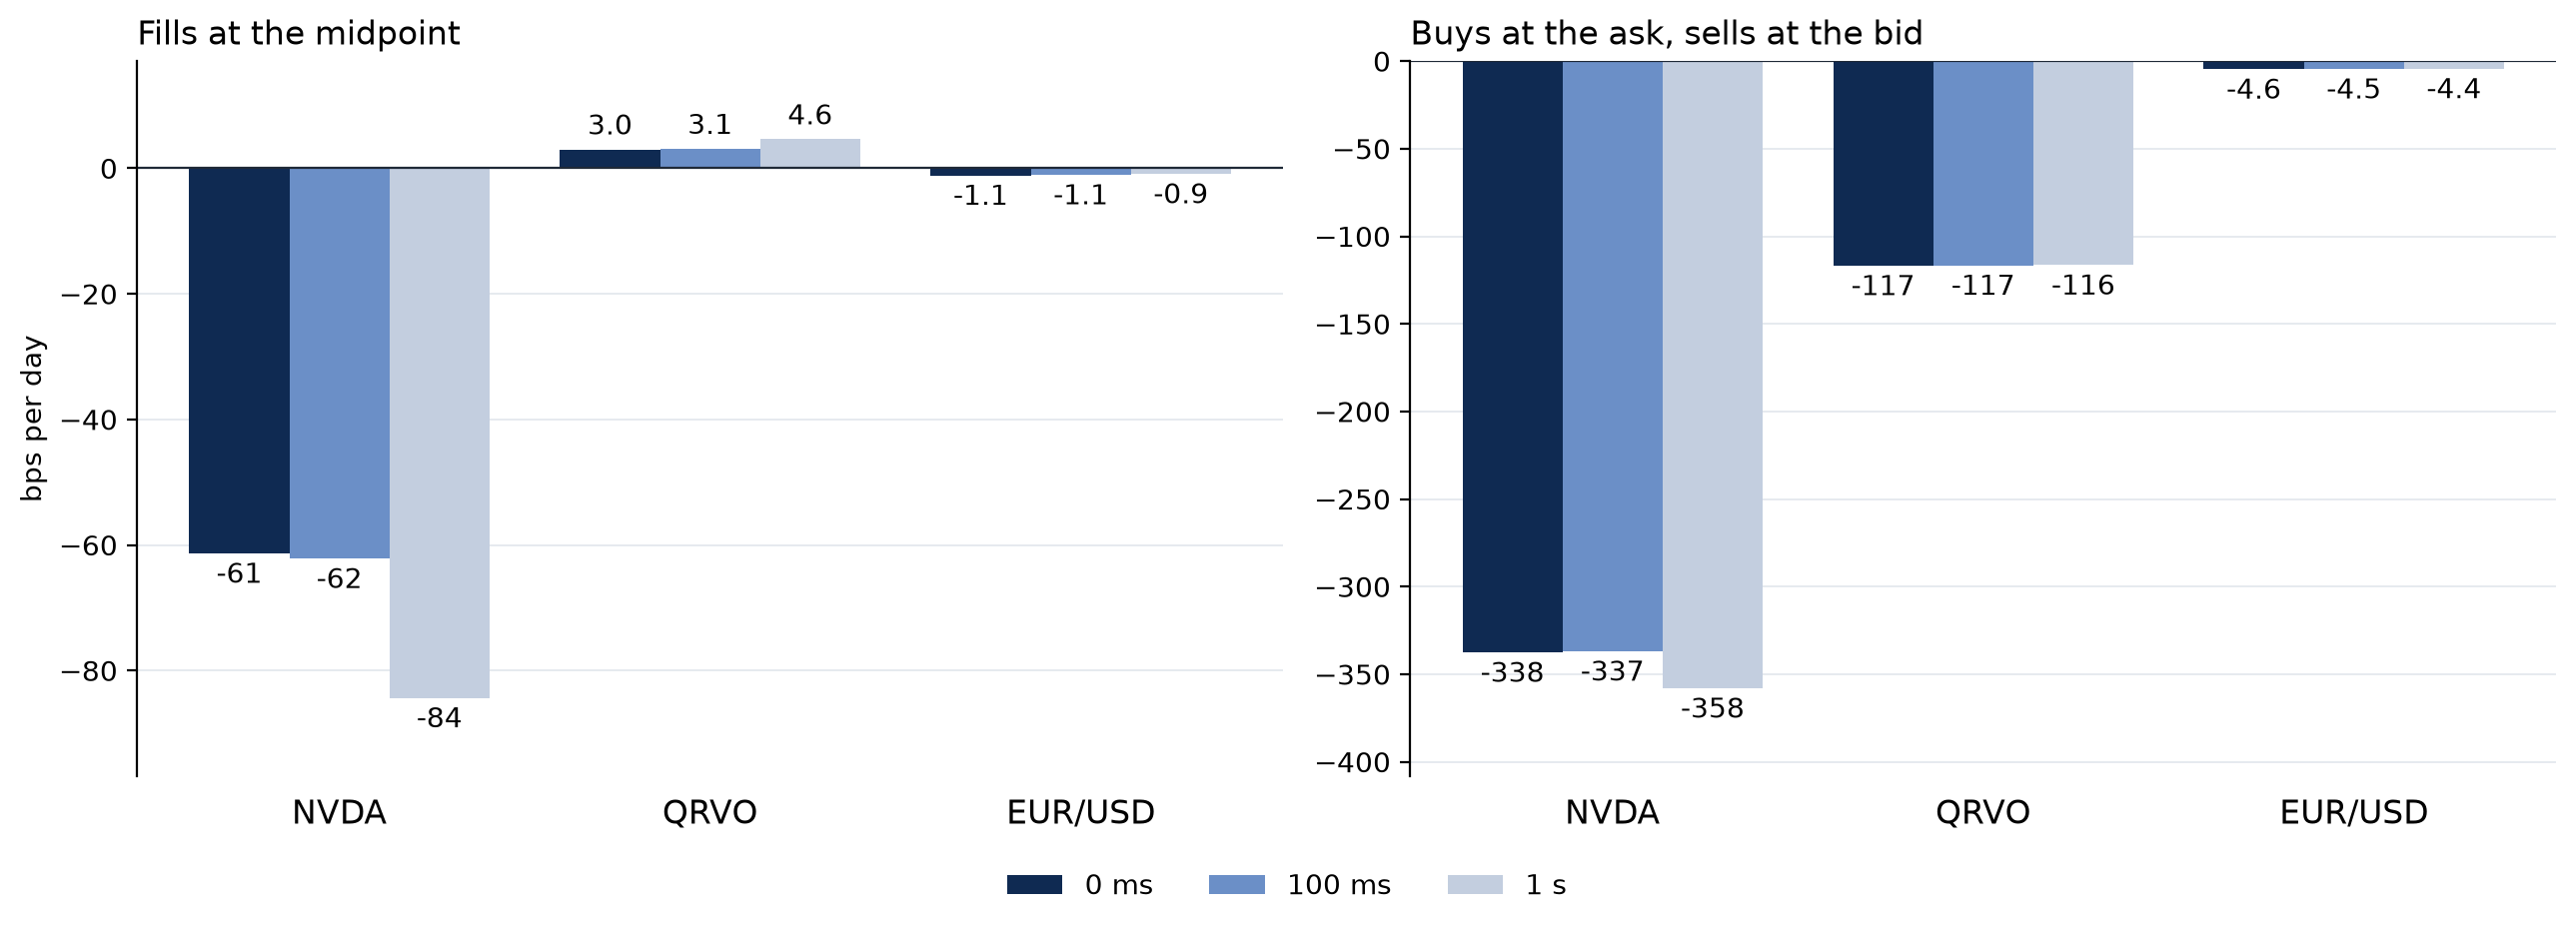
\includegraphics[width=\textwidth]{ma_delay.png}
\caption{MA signal, average daily return by delay. Left: fills at the midpoint. Right: buys at the ask, sells at the bid.}
\label{fig:ma}
\end{figure}

\noindent The rule loses money in all three assets and at every delay. With fills at the touch it loses 43\% of the book in NVDA, 17\% in QRVO and 0.7\% in EUR/USD. It also has no gross return to begin with. With fills at the midpoint it still loses 10\% in NVDA and 0.2\% in EUR/USD. The gain of 0.5\% in QRVO rests on 63 round trips and is positive on only 8 of the 16 days, so we treat it as zero.\\

\noindent In NVDA the rule makes about 260 round trips per day and holds each position for about a minute. It loses 1.3 basis points per round trip at the touch, of which 0.25 basis points are lost before the spread and about 1.1 basis points are the spread itself. Only 27\% of the round trips make money. This is the usual weakness of a trend-following rule on short intervals. A crossover is confirmed only after part of the move has taken place, and when the price turns back instead of continuing, the rule exits at a loss. The gross result is also concentrated in a few days. With fills at the midpoint the rule gains 6.4\% on March 11 alone and is positive on 6 of the 16 days, and with fills at the touch March 11 is the only profitable day. Its daily returns at the midpoint have a correlation of 0.83 with those of the SR rule on the one second interval, which we present in the next section, so the two trend-following rules gain and lose on the same days.\\

\noindent QRVO shows a different problem. The band of 16.85 basis points is crossed only about four times per day, and the positions last six seconds on average. Of the 63 round trips a single one makes money at the touch. The rule loses 30 basis points per round trip at the touch while it gains 0.8 at the midpoint, so it pays about 31 basis points in spread on each round trip, more than four times the median spread of 7.1 basis points. For the short average to move this far from the long one within a few seconds the midpoint has to jump. The size of the spread paid is what we would expect if the midpoint jumps because the quote on one side is withdrawn, which widens the spread at the same time. The rule then trades at the moments when crossing the spread is most expensive. About a third of the loss for the month comes from one day, March 11, when the book loses 5.9\%.\\

\noindent In EUR/USD the band is crossed about five times per day and not at all on two of the 16 days. The loss is 0.9 basis points per round trip at the touch, of which 0.7 is the spread, about one and a half times the median spread of 0.46 basis points. With 84 round trips in total the rule is close to inactive, and its result says little about the asset.\\

\noindent Delay has almost no effect on this rule. At 100 ms the total return changes by at most 0.1 percentage points in any asset and for either fill, and the sign is mixed. In NVDA the delayed return is lower on 9 of the 16 days at the touch, and the Wilcoxon test of Section~\ref{sec:cod} gives a $p$-value of 1.00. In QRVO a delay of 100 ms changes the daily return on one day out of 16, because the quote in effect 100 ms after the signal is almost always the quote that was in effect at the signal. A delay of one second has a visible effect only in NVDA, where the total return falls from $-42.57\%$ to $-44.44\%$ at the touch and from $-9.85\%$ to $-13.05\%$ at the midpoint. This is 20 basis points per day at the touch and 23 at the midpoint, with the delayed return lower on 10 of the 16 days, and it is significant at the 10\% level only at the midpoint. Per round trip it is 0.08 basis points, against 1.1 basis points paid in spread. In QRVO and EUR/USD a delay of one second improves the return by 0.3 basis points per day at the touch, which is not different from zero.\\

\noindent The reason is the horizon of the signal. The long average covers 30 to 120 seconds, so the signal at one second differs from the signal a second earlier by a single observation, and the position is then held for between six seconds and a minute. A delay of 100 ms is a tenth of the sampling interval and a small fraction of the holding period. Only in NVDA, where the midpoint changes about 23 times per second, is the price one second after the crossover different enough to matter. There it tends to have moved further in the direction of the order, so the late order gets a worse price. That a losing rule is hurt by delay differs from the paper, where only profitable rules are affected, but with 16 days the evidence for it is weak.


\subsection{Support and Resistance signal}
The Support and Resistance rule trades on breakouts from the recent price range. We follow equation (7) of Scholtus and van Dijk (2012). The day is divided into intervals of fixed length, and $m_t$ is the midpoint at the end of interval $t$. Let $m^{\max}_t$ and $m^{\min}_t$ be the highest and lowest midpoint reached during interval $t$. The resistance and support levels are the highest and lowest midpoint over the previous $l$ intervals,
\begin{equation}
R_t = \max(m^{\max}_{t-1}, \dots, m^{\max}_{t-l}), \qquad S_t = \min(m^{\min}_{t-1}, \dots, m^{\min}_{t-l}),
\end{equation}
and the signal is
\begin{equation}
SR_t =
\begin{cases}
\phantom{-}1 & \text{if } m_t > (1+b)\,R_t \\
-1 & \text{if } m_t < (1-b)\,S_t \\
SR_{t-1} & \text{otherwise.}
\end{cases}
\end{equation}
The rule goes long when the midpoint breaks above the resistance level and short when it breaks below the support level, and it keeps its position until the opposite level is broken. It starts each day flat, so after the first breakout of the day it is always in the market, and all positions are closed at the end of the day. The paper also applies a delay parameter $d$ and a minimum holding period $h$ to the raw signal. We use the raw signal, which corresponds to $d = 0$ and no minimum holding period.
 
For the parameters we take the shortest interval length of the paper, 30 seconds, with a lookback of $l = 60$ intervals and a band of $b = 0$. The levels are therefore the high and low of the previous 30 minutes. Since a delay of at most one second is short relative to a 30 second interval, we also run the same rule on a one second interval. Here the levels are the high and low of the previous minute. The parameters are the same for all three assets and were fixed in advance and not fitted to the data. Results are reported on the same 16 trading days as we will use in the OFI signal (March 10 to 31). Table~\ref{tab:sr} reports the total return on \$1,000,000 for each delay, and Figure~\ref{fig:sr} shows the average daily returns.
 
\begin{table}[H]
\centering
\begin{tabular}{lllrrrrr}
\toprule
 & & & \multicolumn{3}{c}{Total return (\%)} & \multicolumn{2}{c}{Cost of delay (pp)} \\
Interval & Asset & Fill & 0 ms & 100 ms & 1 s & 100 ms & 1 s \\
\midrule
30 s & NVDA    & mid   & $-2.42$ & $-2.52$ & $-2.31$ & $0.10$ & $-0.11$ \\
     &         & touch & $-3.57$ & $-3.62$ & $-3.46$ & $0.05$ & $-0.11$ \\
     & QRVO    & mid   & $21.91$ & $21.88$ & $21.79$ & $0.03$ & $0.12$ \\
     &         & touch & $12.35$ & $12.28$ & $12.19$ & $0.06$ & $0.16$ \\
     & EUR/USD & mid   & $-1.14$ & $-1.12$ & $-1.07$ & $-0.02$ & $-0.07$ \\
     &         & touch & $-1.79$ & $-1.76$ & $-1.70$ & $-0.04$ & $-0.09$ \\
\midrule
1 s  & NVDA    & mid   & $-18.16$ & $-19.01$ & $-20.98$ & $0.85$ & $2.82$ \\
     &         & touch & $-42.89$ & $-43.14$ & $-44.64$ & $0.25$ & $1.74$ \\
     & QRVO    & mid   & $128.04$ & $127.14$ & $106.74$ & $0.90$ & $21.30$ \\
     &         & touch & $-81.93$ & $-82.33$ & $-84.47$ & $0.40$ & $2.54$ \\
     & EUR/USD & mid   & $-1.03$ & $-0.76$ & $-0.34$ & $-0.27$ & $-0.69$ \\
     &         & touch & $-16.68$ & $-16.34$ & $-15.39$ & $-0.34$ & $-1.28$ \\
\bottomrule
\end{tabular}
\caption{SR signal, March 10 to 31, 2025. On the 30 second interval the signal makes 104 round trips in NVDA, 95 in QRVO and 104 in EUR/USD, with an average holding time of 53 to 58 minutes. On the one second interval it makes 3,276, 2,493 and 2,512 round trips, with an average holding time of about two minutes.}
\label{tab:sr}
\end{table}
\begin{figure}[H]
\centering
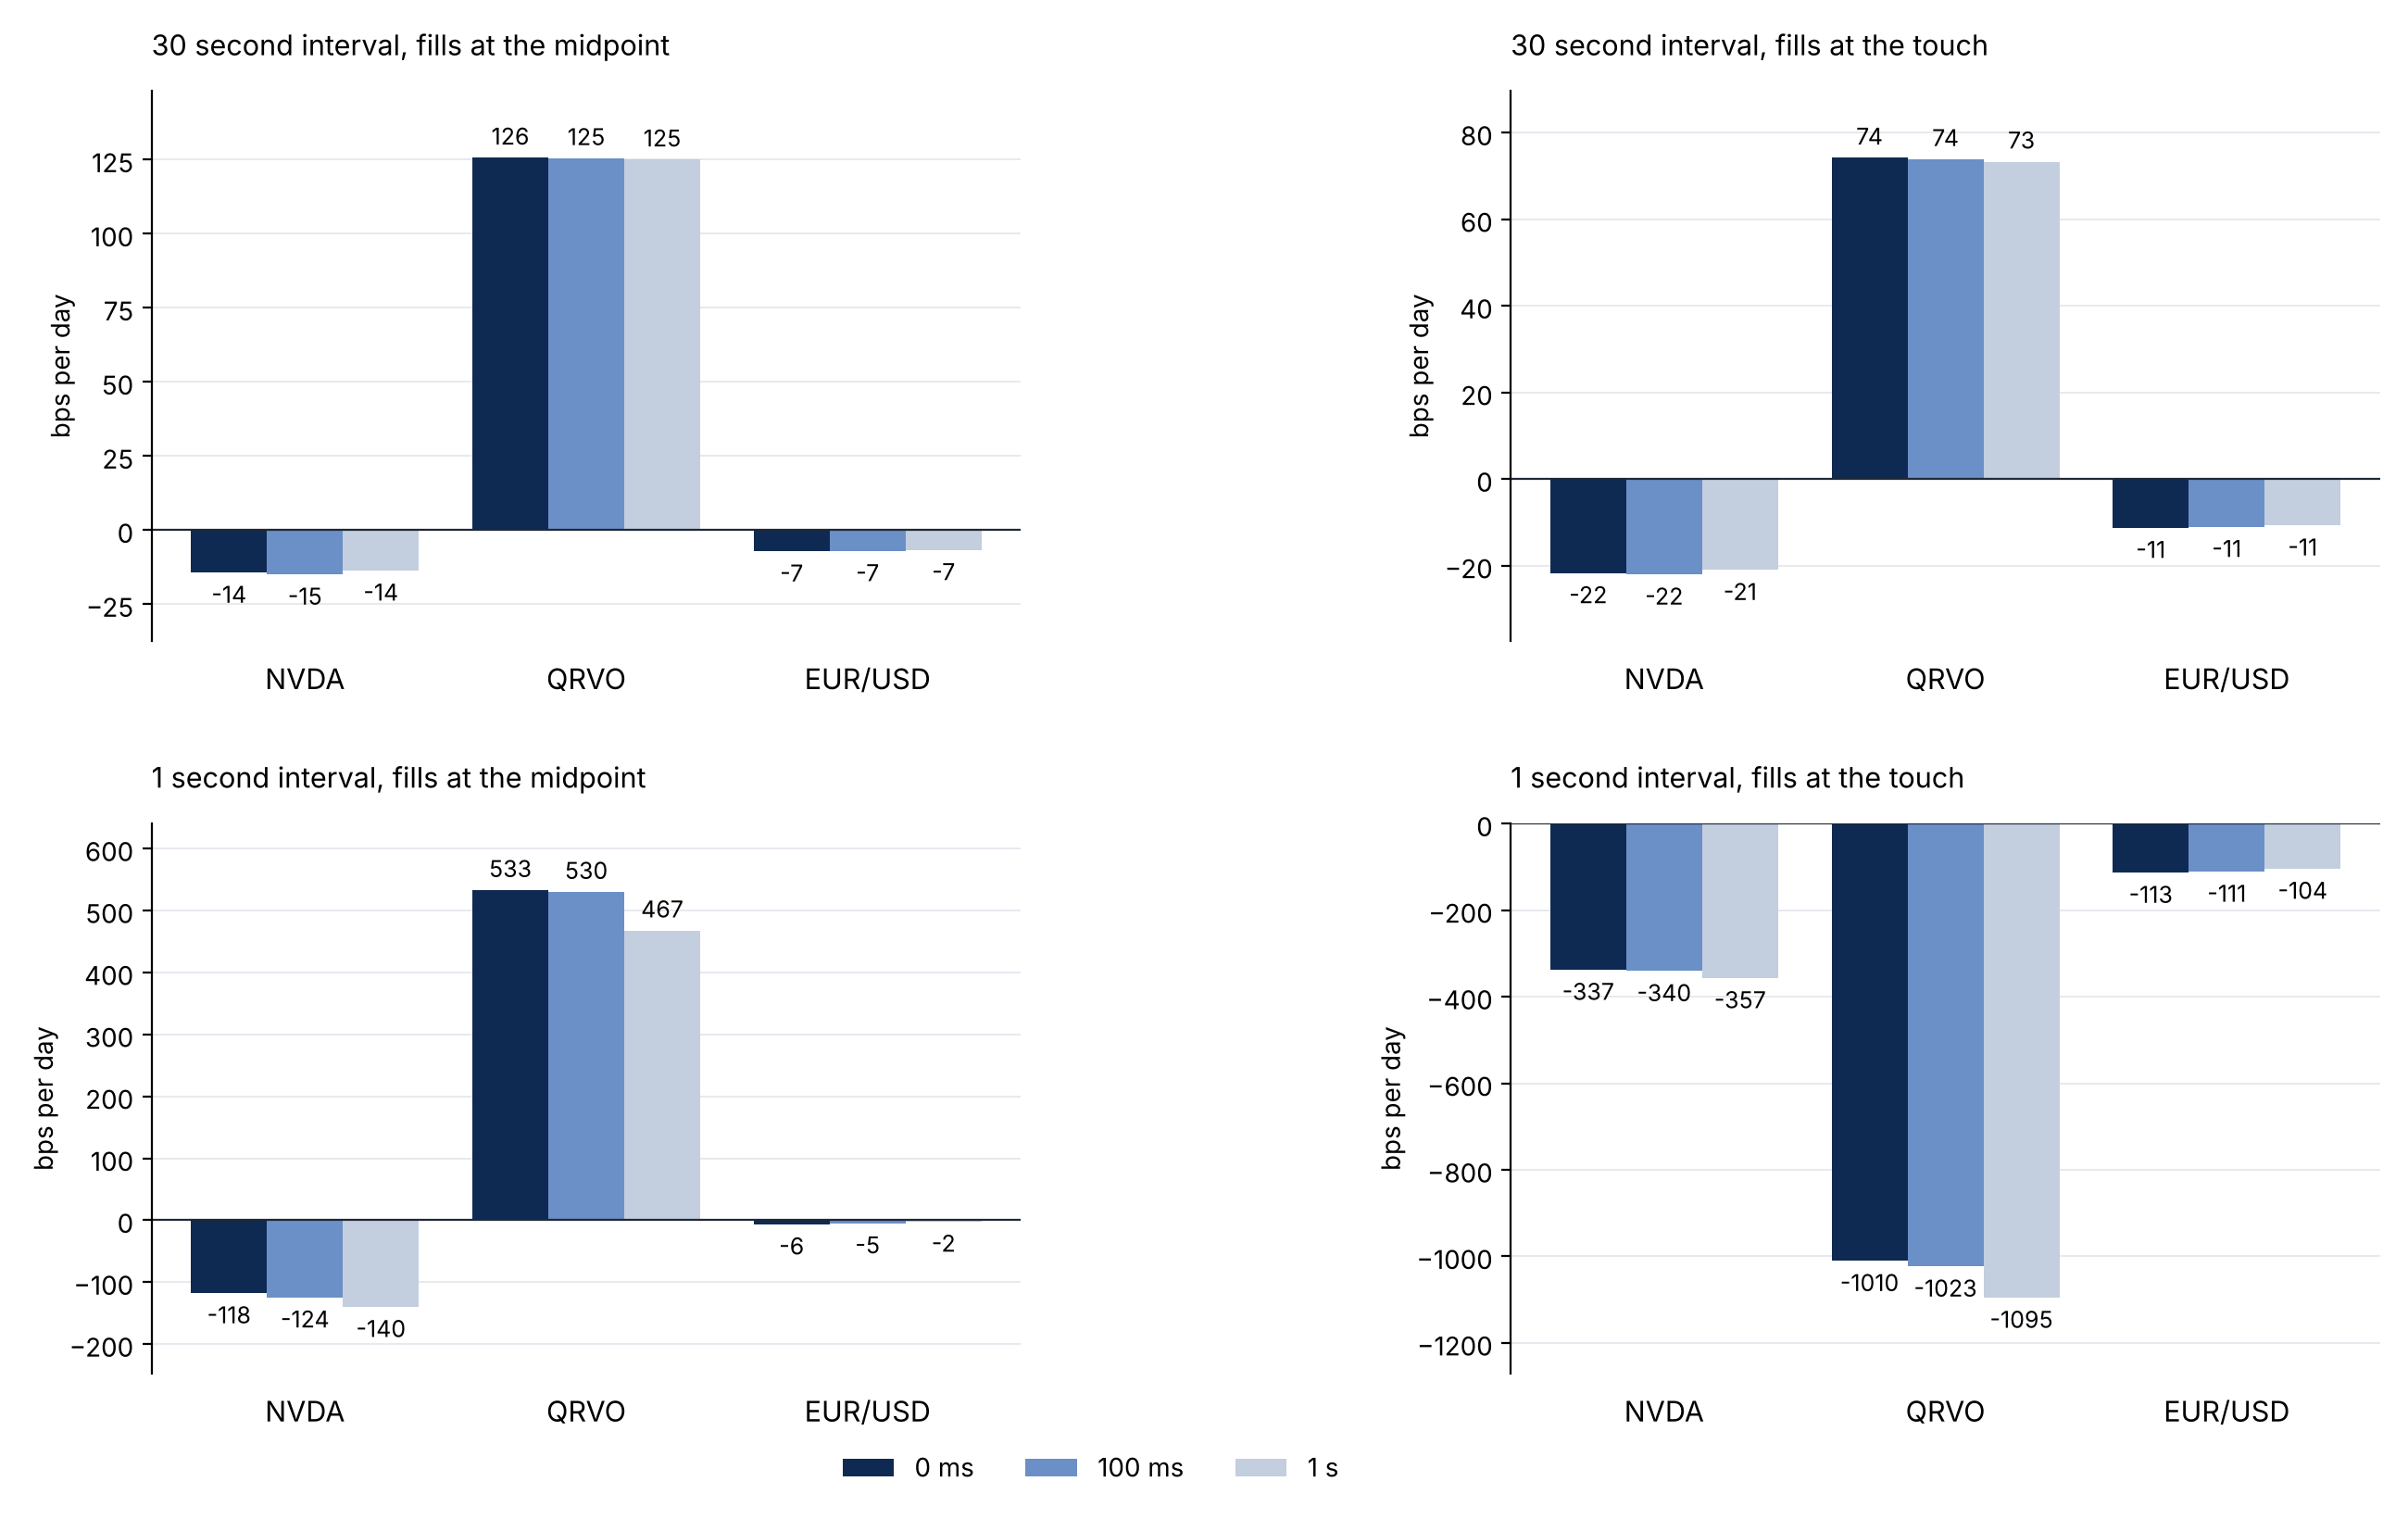
\includegraphics[width=\textwidth]{sr_delay.png}
\caption{SR signal, average daily return by delay. Top: 30 second interval. Bottom: one second interval. Left: fills at the midpoint. Right: buys at the ask, sells at the bid.}
\label{fig:sr}
\end{figure}
 
On the 30 second interval the rule trades about six times per day and holds each position for close to an hour. It loses a small amount in NVDA and EUR/USD and earns 12\% in QRVO after paying the spread, or about 12 basis points per round trip. The QRVO result rests on 95 round trips and the daily return is positive on 12 of the 16 days, so we do not read it as evidence of a reliable profit. It also depends on our assumption that the whole book is filled at the best quote, which is least realistic for QRVO.
 
Delay has no effect on this version of the rule. The cost of delay is below 0.2 percentage points for every asset, both delays and both fill assumptions, and its sign is mixed. The average daily differences are all below one basis point. In QRVO a delay of 100 ms changes the return on only 2 of the 16 days, because the quote that is in effect 100 ms after the signal is almost always the quote that was in effect at the signal. The paper does find a significant effect of delay for profitable rules on the 30 second interval, but a small one, about 2\% of the return with instant execution for SPY. Our estimate for QRVO, the one asset where the rule is profitable, is of the same order, with a delay of one second costing about 1\% of the average daily return at the touch. With one rule and 16 days we cannot distinguish an effect of this size from zero, whereas the paper averages over thousands of rules and nine months. With six trades per day and holding periods of an hour, a price change during the delay is small relative to the price change during the trade.
 
The one second interval gives a different picture. The rule now trades about 150 to 200 times per day and pays the full spread each time, so with fills at the touch it loses between 17\% and 82\% of the book. With fills at the midpoint only QRVO has a positive gross return, about 3.4 basis points per round trip against a median spread of 7.1 basis points. As for the OFI signal, this gain is visible at the midpoint but cannot be earned by an order that crosses the spread.
 
On this interval delay starts to matter, but only at one second and only where there is a gross return to lose. In QRVO a delay of one second costs 65 basis points per day with fills at the midpoint, about 12\% of the gross return, and the delayed return is lower on 15 of the 16 days (paired $t$-statistic 4.3). A delay of 100 ms costs 3 basis points per day, which is not significant. In NVDA the rule loses money before the spread and the cost of delay, 22 basis points per day at one second, is not significant ($t$-statistic 1.5). This matches the finding of the paper that delay hurts rules that are profitable without delay and leaves losing rules unaffected.
 
EUR/USD behaves differently. Here delay improves the return. With fills at the touch a delay of one second raises the average daily return by 9 basis points, and the delayed return is higher on all 16 days. A breakout of the one minute range in EUR/USD is therefore followed by a slightly better price a second later, either because part of the move is reversed or because the spread is wider at the moment of the breakout. The effect is small, but it means that for this rule and this asset there is no reward for being fast.

\subsection{Order flow imbalance signal}

MA and SR are computed from past midpoints on a fixed clock. Scholtus and van Dijk (2012) note in their conclusion that speed is likely to matter more for event based rules that react to the order book. We therefore add a signal of that type. Order flow imbalance (OFI), introduced by Cont, Kukanov and Stoikov (2014), it measures the net buying pressure at the best quotes and is known to move closely with short horizon price changes. It only needs the top of the book, so the same definition applies to both stocks and to the EUR/USD future.\\

\noindent The OFI is defined by letting $P^b_n, q^b_n$ be the best bid price and size after the $n$-th book update, and $P^a_n, q^a_n$ the best ask price and size. Each update contributes
\begin{equation}
e_n = \underbrace{\begin{cases} q^b_n & P^b_n > P^b_{n-1} \\ q^b_n - q^b_{n-1} & P^b_n = P^b_{n-1} \\ -q^b_{n-1} & P^b_n < P^b_{n-1} \end{cases}}_{\text{change in buying pressure}}
\;-\;
\underbrace{\begin{cases} q^a_n & P^a_n < P^a_{n-1} \\ q^a_n - q^a_{n-1} & P^a_n = P^a_{n-1} \\ -q^a_{n-1} & P^a_n > P^a_{n-1} \end{cases}}_{\text{change in selling pressure}}
\end{equation}
so $e_n$ is positive when size is added at the bid or removed from the ask. The signal is the sum over a rolling window of length $W$, scaled by the typical depth $D$ at the touch:
\begin{equation}
x_t = \frac{1}{D} \sum_{n:\; t - W < t_n \le t} e_n .
\end{equation}
The window is computed in event time, so $x_t$ is updated at every book update and again when an update drops out of the window. Scaling by $D$ makes the signal comparable across assets with very different quote sizes. The trading rule follows the imbalance:
\begin{itemize}
\item go long when $x_t > k$ and hold until $x_t \le 0$,
\item go short when $x_t < -k$ and hold until $x_t \ge 0$,
\item otherwise stay flat. All positions are closed at the end of the day.
\end{itemize}

\noindent The window is $W = 2$ seconds. The depth $D$ and the threshold $k$ are set on the first week of the sample (March 3 to 7) and then held fixed, where $D$ is the average size at the best bid and ask, and $k$ is the 95th percentile of $|x_t|$ across all updates, so the rule only trades on the strongest 5\% of imbalances. Results are reported on the remaining 16 trading days. Table~\ref{tab:ofi_params} shows the calibrated values.

\begin{table}[H]
\centering
\begin{tabular}{lrrr}
\hline
 & NVDA & QRVO & EUR/USD \\
\hline
Depth $D$ & 722.6 shares & 163.5 shares & 20.5 contracts \\
Threshold $k$ & 18.64 & 9.80 & 9.49 \\
\hline
\end{tabular}
\caption{OFI parameters, calibrated on March 3 to 7, 2025.}
\label{tab:ofi_params}
\end{table}

\noindent Table~\ref{tab:ofi_results} reports the total return on \$1,000,000 over the 16 days for each delay, with fills at the midpoint and at the touch.

\begin{table}[H]
\centering
\begin{tabular}{llrrrrr}
\hline
 & & \multicolumn{3}{c}{Total return (\%)} & \multicolumn{2}{c}{Cost of delay (pp)} \\
Asset & Fill & 0 ms & 100 ms & 1 s & 100 ms & 1 s \\
\hline
NVDA & mid & 75.46 & $-6.39$ & $-9.16$ & 81.84 & 84.61 \\
 & touch & $-62.27$ & $-77.23$ & $-78.08$ & 14.95 & 15.81 \\
QRVO & mid & 19.37 & 9.69 & 4.75 & 9.69 & 14.62 \\
 & touch & $-51.39$ & $-56.30$ & $-58.83$ & 4.91 & 7.44 \\
EUR/USD & mid & 1.15 & $-0.24$ & 0.40 & 1.39 & 0.75 \\
 & touch & $-25.16$ & $-26.42$ & $-26.02$ & 1.27 & 0.86 \\
\hline
\end{tabular}
\caption{OFI signal, March 10 to 31, 2025. The signal makes 12,283 round trips in NVDA, 1,288 in QRVO and 5,072 in EUR/USD, with an average holding time of 2.2 to 2.4 seconds.}
\label{tab:ofi_results}
\end{table}

\noindent Two results stand out. First, the signal has predictive content but is not profitable. With instant execution at the midpoint it earns a positive return on all three assets, so a strong imbalance does predict the direction of the next price move. Once buys pay the ask and sells receive the bid, it loses on all three. The reason is turnover, that is the positions last about two seconds and each round trip pays the full spread. In NVDA the gross gain is about 0.5 basis points per round trip against a median spread of 0.9 basis points, and in QRVO about 1.4 against 7.1. The share of round trips that make money at the touch is 27\% for NVDA, 8\% for QRVO and 5\% for EUR/USD.\\

\noindent Second, the information in the signal is short lived. In NVDA the entire gross return disappears within 100 ms, falling from 75\% to $-6\%$, and waiting a full second costs only another 3 percentage points. The loss is the same in non-compounded terms, were the average daily return at the midpoint falls from 352 basis points to $-41$ at 100 ms. This differs from the paper, where delays below 200 ms have no significant effect on clock based rules, and supports the authors' conjecture that event based rules are more sensitive to speed. It also shows that delay matters here even though the strategy loses money after costs. The paper finds no effect of speed on losing strategies, but in our case the losses come from the spread and not from a poor signal.\\

\noindent The cost of delay in percentage points is smaller at the touch than at the midpoint for NVDA. This is an effect of compounding, that is at the touch the book has already lost most of its capital, so the same loss per trade is applied to a smaller base.

\begin{figure}[H]
\centering
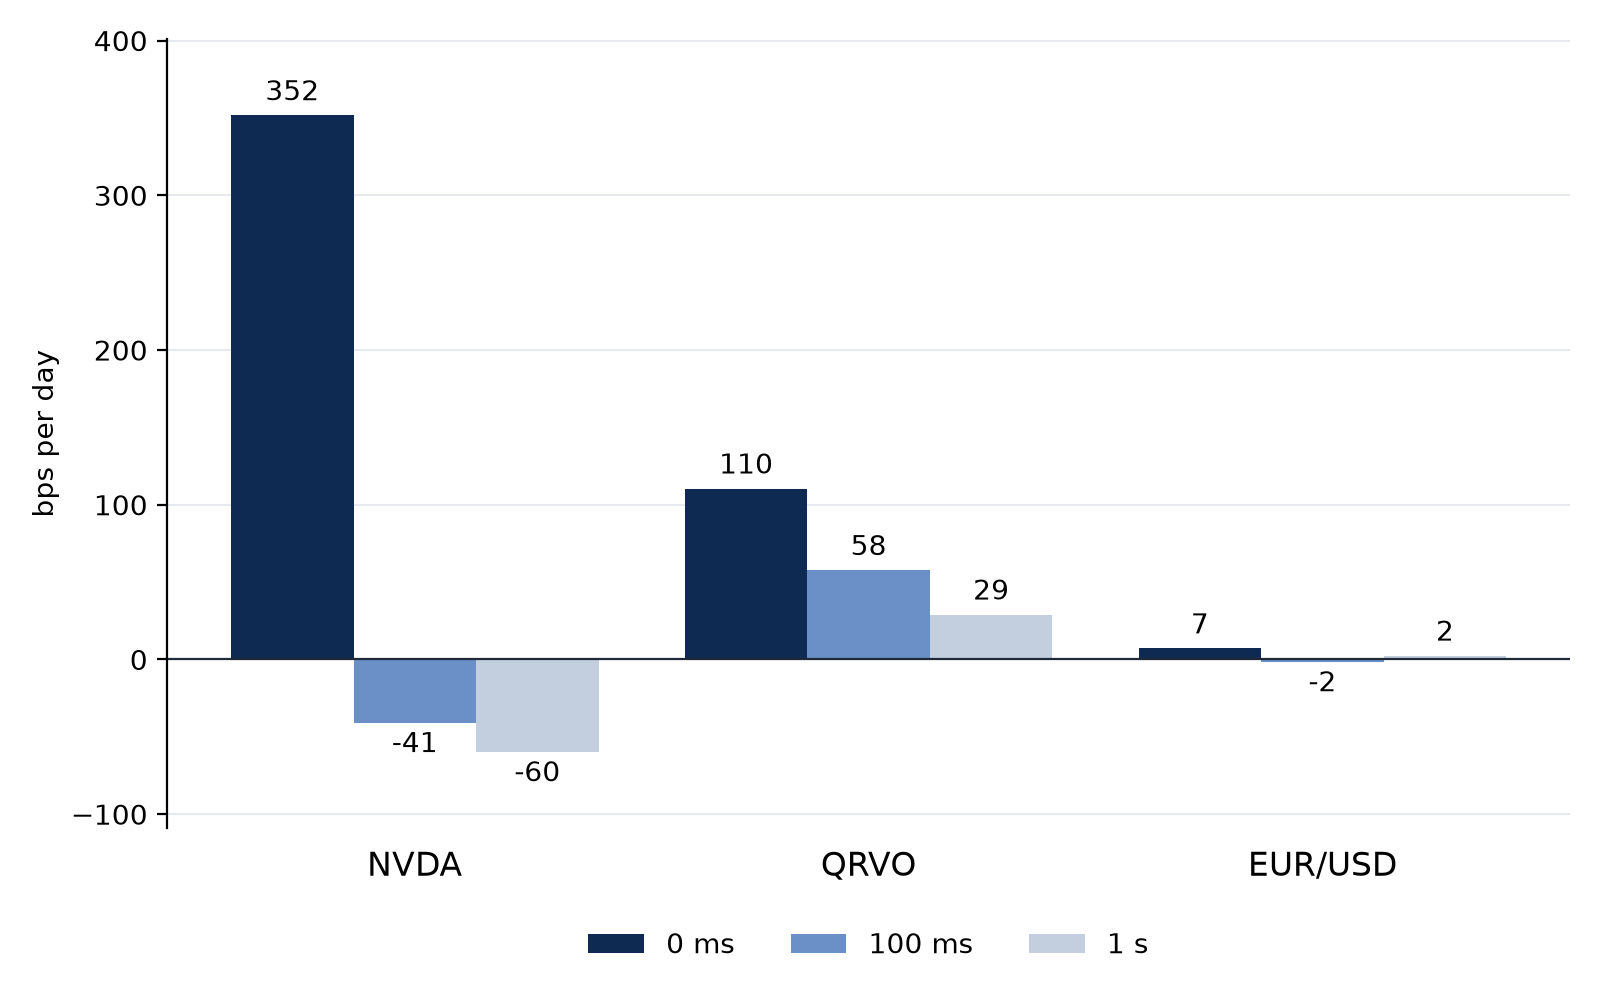
\includegraphics[width=0.48\textwidth]{delay_before_spread.png}
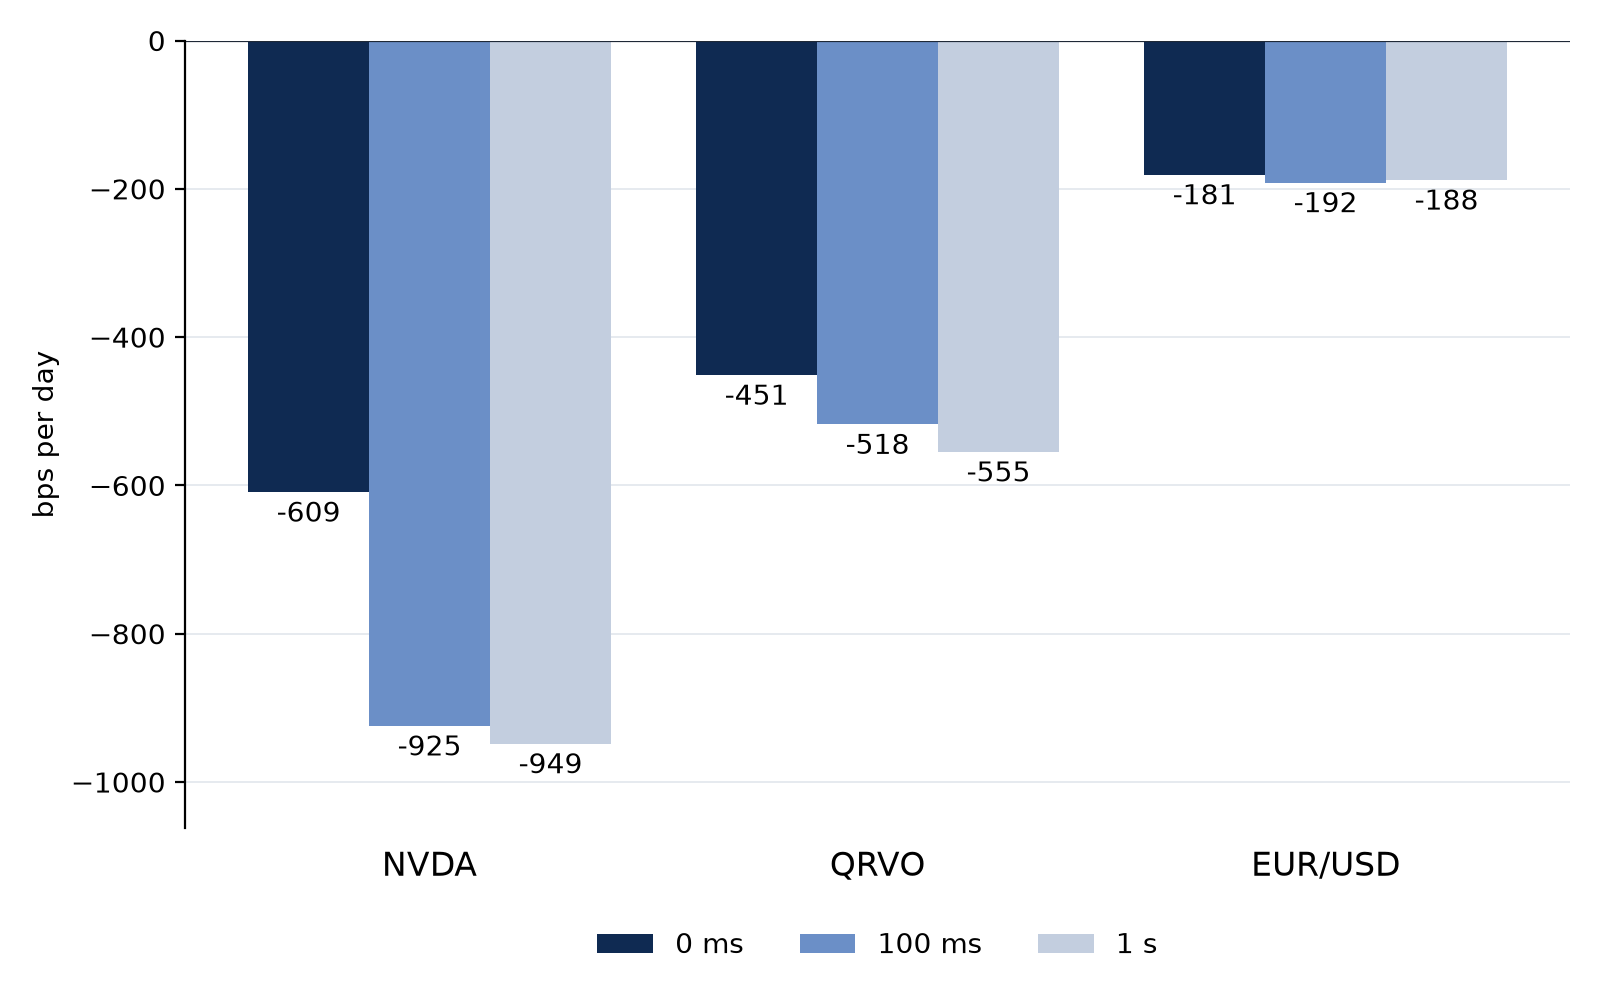
\includegraphics[width=0.48\textwidth]{delay_after_spread.png}
\caption{OFI signal, average daily return by delay. Left: fills at the midpoint. Right: buys at the ask, sells at the bid.}
\label{fig:ofi_delay}
\end{figure}

\noindent The three assets give three different trading environments, and the signal behaves differently in each. In NVDA, where the midpoint changes about twice per 100 ms, the signal fires most often (about 770 round trips per day) and has the largest gross return, but the price adjusts to the imbalance almost immediately, so the edge belongs only to the fastest trader. In QRVO, where the midpoint changes about once every two seconds, the signal fires about 80 times per day and its value decays gradually, were half of the gross return is left at 100 ms and a quarter at 1 second. A slow trader can still capture part of the move, but the wide spread makes the signal the least tradeable after costs. In EUR/USD the gross return is close to zero at every delay and the effect of delay is not monotone, so we cannot distinguish it from noise. One possible reason is that price discovery in EUR/USD is shared with the spot market, so the top of the futures book shows only part of the order flow.\\

\noindent Following the paper, we also split the 16 days for each asset into a high and a low volatility half, using the realized volatility of one minute midpoint returns. Table~\ref{tab:ofi_vol} reports average daily returns with fills at the midpoint.

\begin{table}[H]
\centering
\begin{tabular}{llrrrr}
\hline
 & & Realized vol. & Return at 0 ms & \multicolumn{2}{c}{Cost of delay} \\
Asset & Days & (bps) & (bps per day) & 100 ms & 1 s \\
\hline
NVDA & high vol. & 318.1 & 394.0 & 484.0 & 505.8 \\
 & low vol. & 197.6 & 309.5 & 301.1 & 317.2 \\
QRVO & high vol. & 228.1 & 157.9 & 69.4 & 109.3 \\
 & low vol. & 172.0 & 63.1 & 36.1 & 53.6 \\
EUR/USD & high vol. & 31.7 & 9.6 & 9.7 & 7.7 \\
 & low vol. & 25.5 & 4.7 & 7.6 & 1.6 \\
\hline
\end{tabular}
\caption{OFI signal on high and low volatility days (8 days each), fills at the midpoint. Cost of delay is the return at 0 ms minus the return with delay, in basis points per day.}
\label{tab:ofi_vol}
\end{table}

\noindent The signal is stronger when markets are volatile. The return with instant execution is higher on high volatility days for all three assets, and more than twice as high for QRVO and EUR/USD. The cost of delay in basis points is also higher on those days, since prices move further during the delay. In NVDA the cost exceeds the gross return on volatile days, so a trader who is 100 ms late loses about 90 basis points per day, while on calm days the same delay only brings the return to zero. Acting late on a stale imbalance is therefore most costly exactly when the signal is most valuable.\\ 

\noindent Relative to the return at 0 ms the picture is mixed. In QRVO a delay of 100 ms removes 44\% of the gross return on volatile days and 57\% on calm days, which matches the paper's finding that speed matters more when volatility is low. In NVDA the ordering is reversed. The EUR/USD figures are too small to interpret. With eight days in each group these differences are indicative only.


\subsection{Cost of delay}
\label{sec:cod}

This section puts the three signals side by side. Figure 6 of Scholtus and van Dijk (2012) shows the change in the performance of a strategy when its execution is delayed, relative to instant execution, and tests the difference with a Wilcoxon signed-rank test. We make the same comparison for each signal and asset. Let $r_{i,d}$ be the return on the book on test day $i$ with delay $d$, in basis points. The cost of delay is
\begin{equation}
C_d = \frac{1}{N} \sum_{i=1}^{N} \left( r_{i,0} - r_{i,d} \right),
\end{equation}
with $N = 16$ days, so a positive value means that the delay loses money. We test it with a two-sided Wilcoxon signed-rank test on the 16 pairs of daily returns. With 16 days the smallest possible $p$-value is 0.00003, which is reached when the delayed return is lower on every day.\\

\noindent We use a difference in returns and not the relative change of the paper, because our returns with instant execution are often negative or close to zero, and a relative change then changes sign and loses its meaning. Since every run starts from the same \$1,000,000, a difference in basis points of the book can be compared across assets and signals. In this section SR refers to the rule on the one second interval, so that MA and SR run on the same clock. The 30 second version has no measurable cost of delay (Table~\ref{tab:sr}).\\

\noindent Table~\ref{tab:pnl} collects the P\&L reports for the 27 combinations of signal, asset and delay, with buys at the ask and sells at the bid. The last column gives the total return of the same run with fills at the midpoint.

\begin{table}[H]
\centering
\small
\setlength{\tabcolsep}{5pt}
\begin{tabular}{lllrrrrrrr}
\toprule
 & & & Final value & P\&L & Return & Daily & Hit rate & Max. DD & Return at \\
Signal & Asset & Delay & (\$) & (\$) & (\%) & (bps) & (\%) & (\%) & mid (\%) \\
\midrule
MA & NVDA & 0 ms & $574{,}271$ & $-425{,}729$ & $-42.57$ & $-337.6$ & $27.1$ & $-42.57$ & $-9.85$ \\
 &  & 100 ms & $575{,}043$ & $-424{,}957$ & $-42.50$ & $-336.9$ & $27.0$ & $-42.60$ & $-9.95$ \\
 &  & 1 s & $555{,}617$ & $-444{,}383$ & $-44.44$ & $-358.0$ & $27.4$ & $-44.44$ & $-13.05$ \\
\addlinespace[2pt]
 & QRVO & 0 ms & $827{,}194$ & $-172{,}806$ & $-17.28$ & $-116.8$ & $1.6$ & $-17.28$ & $0.48$ \\
 &  & 100 ms & $827{,}428$ & $-172{,}572$ & $-17.26$ & $-116.6$ & $1.6$ & $-17.26$ & $0.49$ \\
 &  & 1 s & $827{,}586$ & $-172{,}414$ & $-17.24$ & $-116.5$ & $1.6$ & $-17.24$ & $0.74$ \\
\addlinespace[2pt]
 & EUR/USD & 0 ms & $992{,}629$ & $-7{,}371$ & $-0.74$ & $-4.6$ & $22.6$ & $-0.81$ & $-0.18$ \\
 &  & 100 ms & $992{,}767$ & $-7{,}233$ & $-0.72$ & $-4.5$ & $22.6$ & $-0.79$ & $-0.17$ \\
 &  & 1 s & $993{,}043$ & $-6{,}957$ & $-0.70$ & $-4.4$ & $22.6$ & $-0.77$ & $-0.14$ \\
\midrule
SR & NVDA & 0 ms & $571{,}054$ & $-428{,}946$ & $-42.89$ & $-337.4$ & $31.6$ & $-43.40$ & $-18.16$ \\
 &  & 100 ms & $568{,}561$ & $-431{,}439$ & $-43.14$ & $-340.4$ & $31.8$ & $-43.49$ & $-19.01$ \\
 &  & 1 s & $553{,}646$ & $-446{,}354$ & $-44.64$ & $-356.7$ & $31.3$ & $-44.65$ & $-20.98$ \\
\addlinespace[2pt]
 & QRVO & 0 ms & $180{,}685$ & $-819{,}315$ & $-81.93$ & $-1{,}010.3$ & $23.9$ & $-81.93$ & $128.04$ \\
 &  & 100 ms & $176{,}678$ & $-823{,}322$ & $-82.33$ & $-1{,}023.0$ & $23.8$ & $-82.33$ & $127.14$ \\
 &  & 1 s & $155{,}316$ & $-844{,}684$ & $-84.47$ & $-1{,}095.3$ & $22.9$ & $-84.47$ & $106.74$ \\
\addlinespace[2pt]
 & EUR/USD & 0 ms & $833{,}235$ & $-166{,}765$ & $-16.68$ & $-113.3$ & $22.8$ & $-16.68$ & $-1.03$ \\
 &  & 100 ms & $836{,}616$ & $-163{,}384$ & $-16.34$ & $-110.8$ & $22.8$ & $-16.34$ & $-0.76$ \\
 &  & 1 s & $846{,}053$ & $-153{,}947$ & $-15.39$ & $-103.9$ & $23.2$ & $-15.39$ & $-0.34$ \\
\midrule
OFI & NVDA & 0 ms & $377{,}255$ & $-622{,}745$ & $-62.27$ & $-580.9$ & $27.1$ & $-62.27$ & $75.46$ \\
 &  & 100 ms & $227{,}745$ & $-772{,}255$ & $-77.23$ & $-868.8$ & $22.2$ & $-77.23$ & $-6.39$ \\
 &  & 1 s & $219{,}189$ & $-780{,}811$ & $-78.08$ & $-889.5$ & $23.1$ & $-78.08$ & $-9.16$ \\
\addlinespace[2pt]
 & QRVO & 0 ms & $486{,}063$ & $-513{,}937$ & $-51.39$ & $-437.4$ & $7.9$ & $-51.39$ & $19.37$ \\
 &  & 100 ms & $437{,}013$ & $-562{,}987$ & $-56.30$ & $-500.1$ & $4.5$ & $-56.30$ & $9.69$ \\
 &  & 1 s & $411{,}702$ & $-588{,}298$ & $-58.83$ & $-534.7$ & $3.0$ & $-58.83$ & $4.75$ \\
\addlinespace[2pt]
 & EUR/USD & 0 ms & $748{,}438$ & $-251{,}562$ & $-25.16$ & $-179.3$ & $4.9$ & $-25.16$ & $1.15$ \\
 &  & 100 ms & $735{,}760$ & $-264{,}240$ & $-26.42$ & $-189.7$ & $3.7$ & $-26.42$ & $-0.24$ \\
 &  & 1 s & $739{,}840$ & $-260{,}160$ & $-26.02$ & $-186.4$ & $3.8$ & $-26.02$ & $0.40$ \\
\bottomrule
\end{tabular}
\caption{P\&L reports on \$1,000,000, March 10 to 31, 2025 (16 trading days), buys at the ask and sells at the bid. Daily is the average daily return on the book, hit rate is the share of round trips that make money, and the maximum drawdown is measured on end of day book values. SR is the rule on the one second interval.}
\label{tab:pnl}
\end{table}

\noindent All 27 reports end below \$1,000,000. The final value ranges from \$993,043 for MA in EUR/USD, which hardly trades, to \$155,316 for SR in QRVO. Before the spread the picture is different, with a positive return for OFI in all three assets with instant execution and for SR in QRVO at every delay. The sign of every report is therefore decided by the spread and not by the delay. What the delay decides is how much of the gross return is left. Table~\ref{tab:cod} and Figure~\ref{fig:cod} measure this.

\begin{table}[H]
\centering
\small
\newcommand{\sg}[1]{\rlap{$^{#1}$}}
\setlength{\tabcolsep}{7.5pt}
\begin{tabular}{llrrrrrrrr}
\toprule
 & & \multicolumn{2}{c}{Touch (bps per day)} & \multicolumn{2}{c}{Mid (bps per day)} & \multicolumn{2}{c}{Days lower} & \multicolumn{2}{c}{Per round trip (bps)} \\
Signal & Asset & 100 ms & 1 s & 100 ms & 1 s & 100 ms & 1 s & 100 ms & 1 s \\
\midrule
MA  & NVDA    & $-0.7$ & $20.4$ & $0.8$ & $23.0$\sg{*} & 9 & 10 & $0.00$ & $0.08$ \\
    & QRVO    & $-0.2$ & $-0.3$ & $-0.1$ & $-1.6$ & 0 & 6 & $-0.04$ & $-0.08$ \\
    & EUR/USD & $-0.1$ & $-0.3$ & $-0.1$\sg{*} & $-0.2$ & 3 & 5 & $-0.02$ & $-0.05$ \\
\midrule
SR  & NVDA    & $3.0$ & $19.3$ & $6.8$ & $22.2$ & 10 & 10 & $0.01$ & $0.09$ \\
    & QRVO    & $12.7$\sg{**} & $84.9$\sg{***} & $2.9$ & $65.2$\sg{***} & 13 & 16 & $0.09$ & $0.61$ \\
    & EUR/USD & $-2.5$\sg{***} & $-9.4$\sg{***} & $-1.7$\sg{**} & $-4.4$\sg{**} & 2 & 0 & $-0.02$ & $-0.06$ \\
\midrule
OFI & NVDA    & $287.9$\sg{***} & $308.6$\sg{***} & $398.8$\sg{***} & $417.7$\sg{***} & 16 & 16 & $0.41$ & $0.44$ \\
    & QRVO    & $62.7$\sg{***} & $97.2$\sg{***} & $53.6$\sg{***} & $82.6$\sg{***} & 16 & 16 & $0.83$ & $1.29$ \\
    & EUR/USD & $10.5$\sg{***} & $7.1$\sg{**} & $8.7$\sg{***} & $4.7$ & 16 & 12 & $0.03$ & $0.02$ \\
\bottomrule
\end{tabular}
\caption{Cost of delay, March 10 to 31, 2025. The first four columns give $C_d$ in basis points per day, with fills at the touch and at the midpoint. Stars mark a difference from instant execution at the 10\% ($^{*}$), 5\% ($^{**}$) and 1\% ($^{***}$) level in a two-sided Wilcoxon signed-rank test. Days lower is the number of days out of 16 on which the delayed return at the touch is below the return with instant execution. Per round trip is the difference between the log of the final book value at the touch with instant and with delayed execution, divided by the number of round trips.}
\label{tab:cod}
\end{table}

\begin{figure}[H]
\centering
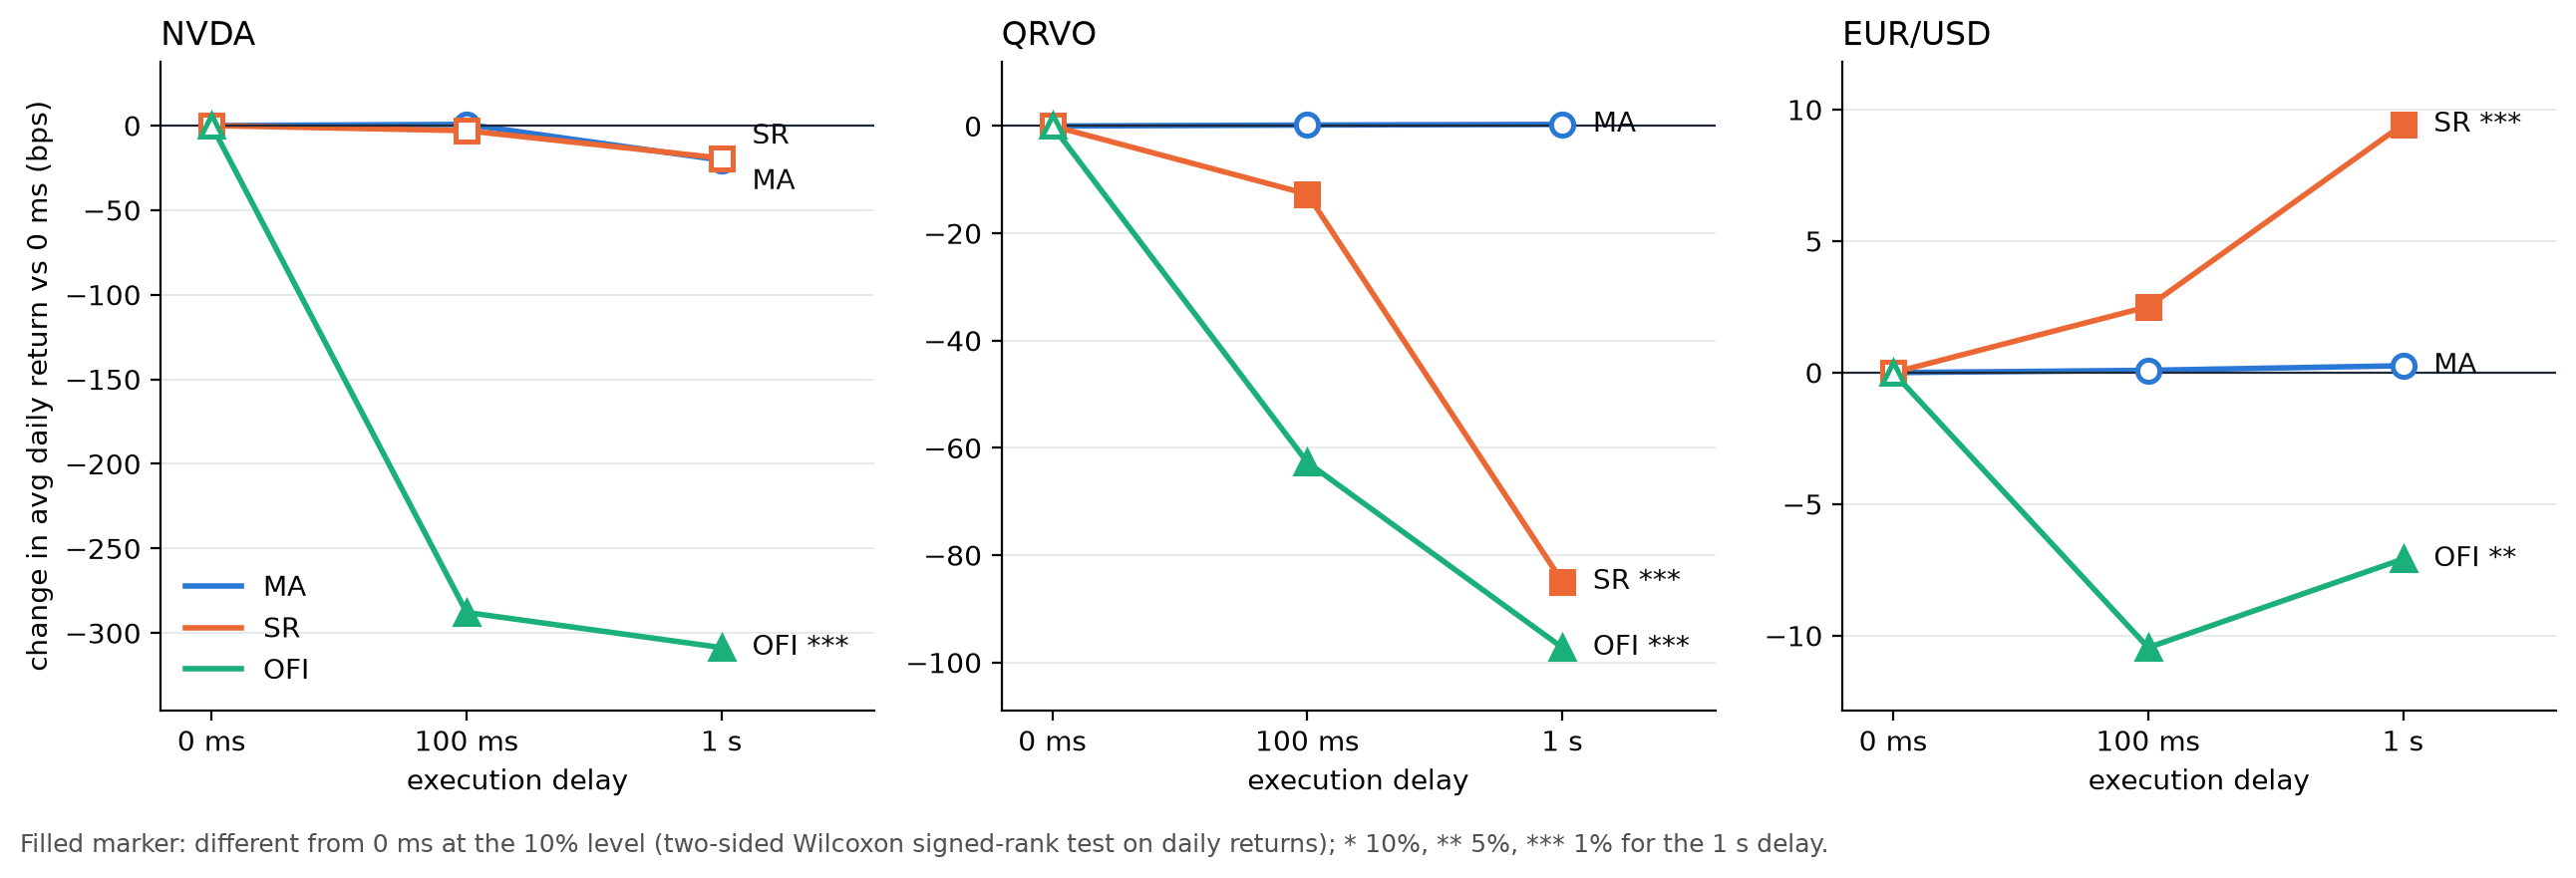
\includegraphics[width=\textwidth]{cost_of_delay_touch.png}\\[6pt]
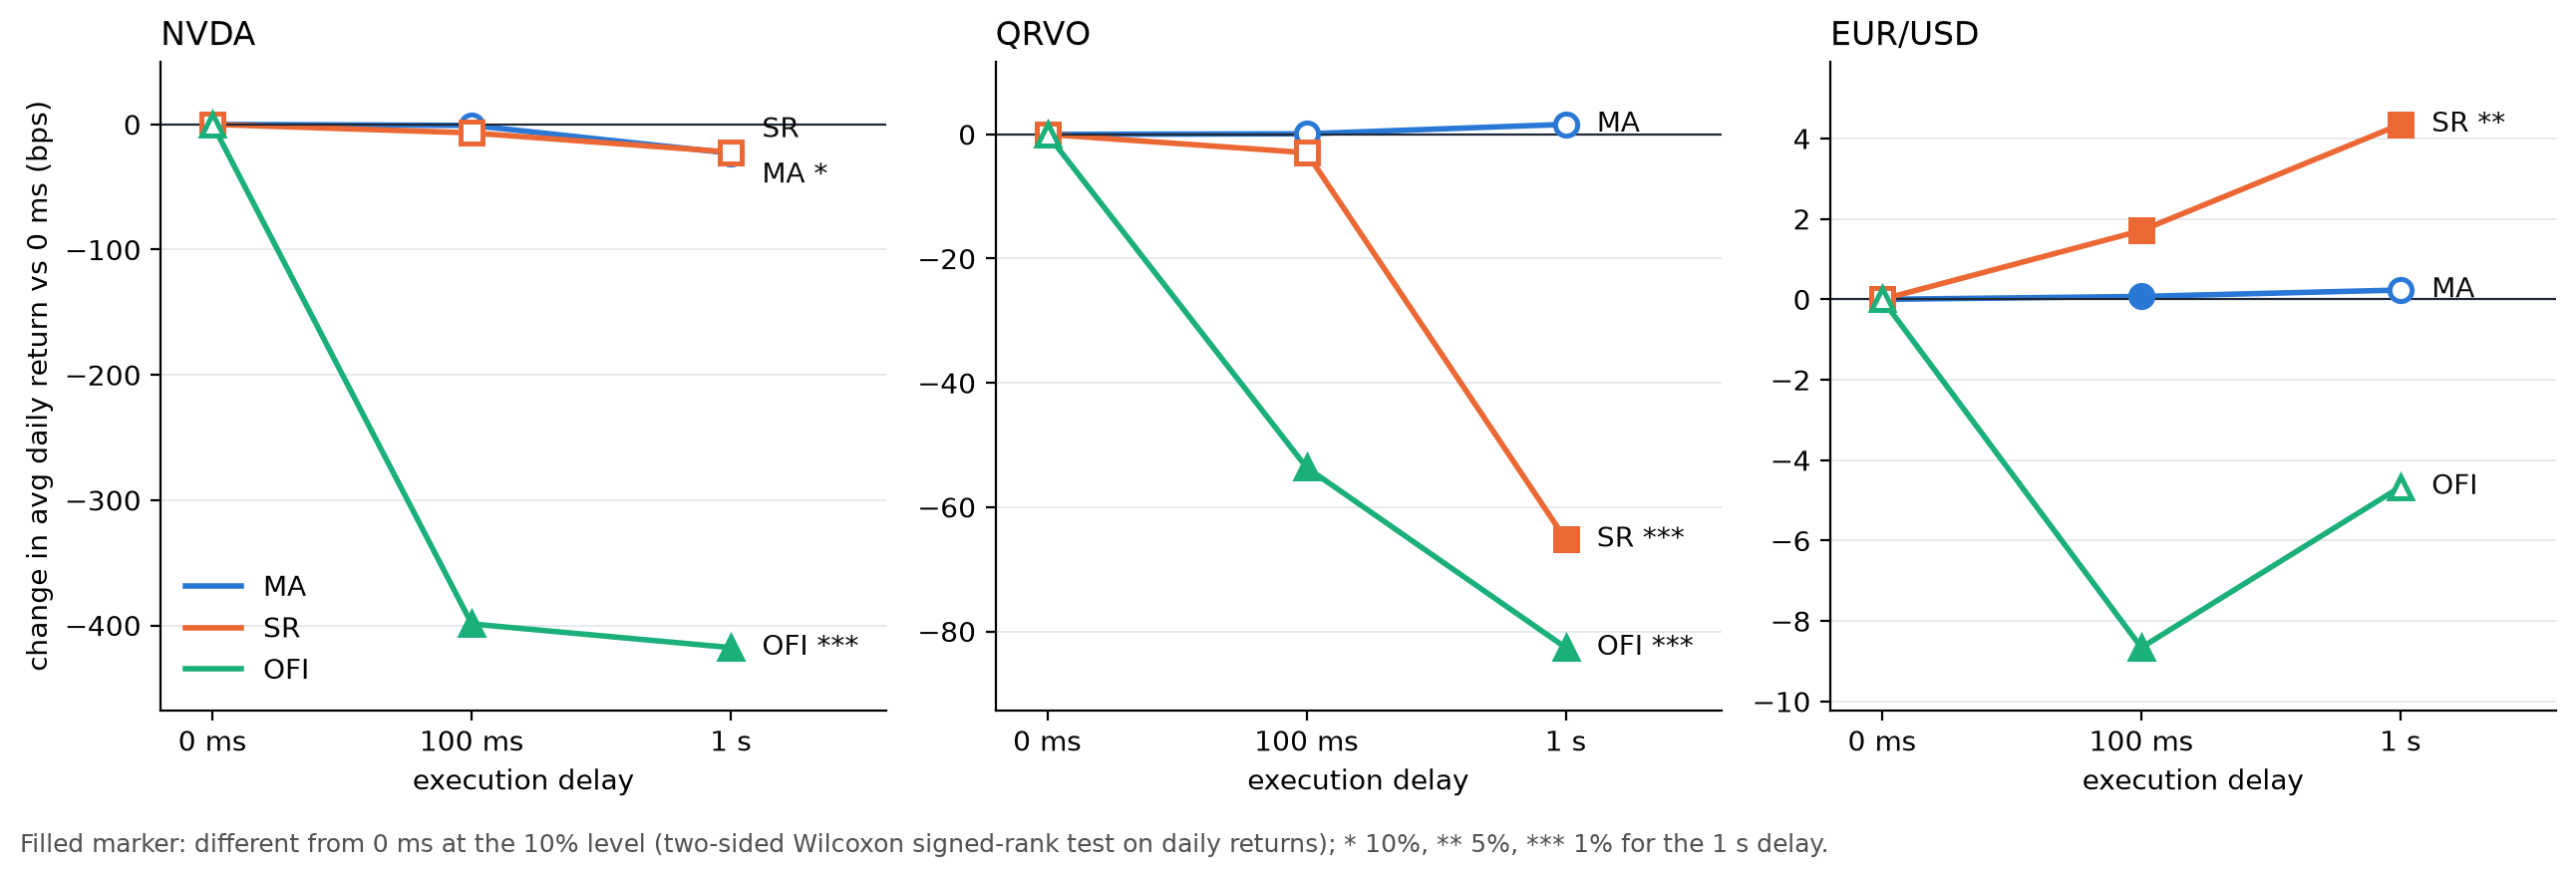
\includegraphics[width=\textwidth]{cost_of_delay_mid.png}
\caption{Change in the average daily return relative to instant execution, our version of Figure 6 of the paper. Top: buys at the ask, sells at the bid. Bottom: fills at the midpoint. A negative value means that the delay lowers the return, so the figure shows $-C_d$.}
\label{fig:cod}
\end{figure}

\noindent The cost of delay is determined first by the type of signal and only then by the asset. Three patterns appear.\\

\noindent First, for the event based OFI signal the cost is large, it is significant in every asset, and most of it arises within the first 100 ms. In NVDA a delay of 100 ms costs 288 basis points per day at the touch, and the delayed return is lower on all 16 days. Waiting a full second adds only 21 basis points, so 93\% of the cost of a one second delay is already incurred after 100 ms. In QRVO the cost is 63 basis points per day at 100 ms and 97 at one second, so about two thirds arises in the first 100 ms and the rest builds up more slowly. In EUR/USD it is 10 basis points at 100 ms and 7 at one second, which is significant but small and does not increase with the delay.\\

\noindent Second, for the two clock based rules the cost appears at one second, which is the length of their sampling interval, and hardly at 100 ms. In NVDA the two rules give almost the same number, 20 basis points per day for MA and 19 for SR at one second with fills at the touch, against 3 or less at 100 ms, and neither is significant at the 5\% level. The clearly significant case is SR in QRVO, where a delay of one second costs 85 basis points per day at the touch and lowers the return on all 16 days. This is also the only clock based rule with a gross return that a delay can take away, 128\% at the midpoint. SR in QRVO is also the one clock based case with a significant cost at 100 ms, 13 basis points per day at the touch. At the midpoint that cost is 3 basis points and not significant, so it comes from the spread paid and not from the price. MA in QRVO and EUR/USD trades four to five times per day and shows no cost at all.\\

\noindent Third, the cost can be negative. For SR in EUR/USD a delay raises the return, by 2.5 basis points per day at 100 ms and 9.4 at one second with fills at the touch, on 14 and on all 16 days. At the midpoint the gain at one second is 4.4 basis points, so about half of it comes from the midpoint moving back after the breakout and the other half from a narrower spread one second later. A rule that is on average wrong at the instant it trades loses less when it trades late.\\

\noindent Which asset is affected most depends on how the cost is measured. Per day it is NVDA, because the OFI signal makes about 770 round trips per day there against 80 in QRVO. Per round trip it is QRVO. A delay of one second costs 1.3 basis points per round trip for OFI in QRVO against 0.4 in NVDA, and 0.6 against 0.1 for SR. A likely reason is that quotes in QRVO move in larger steps relative to the price, as its spread of 7.1 basis points against 0.9 suggests, so a late order that misses a price change loses more. Relative to the gross return the ranking turns around again. With fills at the midpoint, 100 ms removes the whole gross return of OFI in NVDA (399 of 359 basis points per day) and about half of it in QRVO (54 of 112). EUR/USD is the least affected asset by every measure. Its cost never exceeds 11 basis points per day or 0.03 basis points per round trip.\\

\noindent Comparing the two fill assumptions shows what a late order loses. For MA and SR in NVDA the cost is about the same at the midpoint and at the touch (23 and 20 basis points for MA), so the loss comes from the midpoint moving away during the delay and not from the spread. For OFI in NVDA the cost is lower at the touch than at the midpoint, 288 against 399 basis points per day. The spread paid per round trip, measured as the difference between the return per round trip at the midpoint and at the touch, is 1.25 basis points with instant execution and 1.15 with a delay of 100 ms. The spread is thus wider at the instant a strong imbalance appears than 100 ms later, and the fastest trader gives part of the advantage back through the spread. In QRVO it is the other way around. The spread paid rises from 7.0 basis points per round trip with instant execution to 7.3 at one second for OFI, and from 10.2 to 10.4 for SR, so a late order loses on the price and on the spread.\\

\noindent Compared with the paper, our clock based rules behave as it predicts. The paper finds that delay becomes significant from about 200 ms for rules that are profitable without delay and has no effect on losing rules. We find almost no effect at 100 ms for MA and SR, and at one second the significant cost appears in the one case with a gross profit. The OFI signal goes beyond the paper in two ways. Its cost of delay is almost fully present at 100 ms, the shortest delay we test, and it is present although the strategy loses money after the spread. Both follow from the nature of the signal. It reacts to the same order book events that move the price, so its information is gone within the time it takes the quotes to adjust.\\

\noindent In dollar terms, on the \$1,000,000 book a delay of 100 ms lowers the final value of the OFI strategy in NVDA by \$149,510 over the 16 days. A delay of one second lowers the final value of the MA strategy in NVDA by \$18,654 and raises that of SR in EUR/USD by \$12,818. Three remarks apply to these numbers. The dollar and percentage point figures depend on compounding, since a book that has already lost most of its capital loses fewer dollars per trade, which is why we base the comparison on daily returns. Compounding is also why the OFI figures at the midpoint are slightly higher here than in Table~\ref{tab:tick} (399 against 393 basis points for NVDA at 100 ms). Here the book is reinvested after every trade, and there the daily return is not compounded. Finally, the benchmark of 0 ms cannot be reached in practice, so the figures measure the value of the first 100 ms and of the first second after the signal, and not the cost relative to a realistic competitor.


\subsection{Tick frequency and the importance of delay}
Table~\ref{tab:tick} puts the tick frequency of each asset next to the cost of delay of the event based OFI signal and the clock based SR signal. The tick frequencies are those of Table 1, together with the share of quote updates that arrive within 100 ms of the previous update.
 
\begin{table}[h]
\centering
\begin{tabular}{lrrr}
\toprule
 & NVDA & QRVO & EUR/USD \\
\midrule
Midpoint changes per 100 ms & 2.26 & 0.05 & 0.16 \\
Midpoint changes per second & 22.56 & 0.51 & 1.61 \\
Median time between quote updates (ms) & 0.05 & 0.36 & 0.12 \\
Updates within 100 ms of the previous one (\%) & 99.2 & 75.7 & 93.3 \\
\midrule
OFI, cost of 100 ms (bps per day) & 392.6 & 52.8 & 8.7 \\
OFI, cost of 1 s (bps per day) & 411.5 & 81.5 & 4.7 \\
OFI, gross return lost at 100 ms (\%) & 112 & 48 & -- \\
\midrule
SR 1 s interval, cost of 100 ms (bps per day) & 6.8 & 3.0 & $-1.7$ \\
SR 1 s interval, cost of 1 s (bps per day) & 22.2 & 65.2 & $-4.4$ \\
\midrule
SR 30 s interval, cost of 100 ms (bps per day) & 0.6 & 0.2 & $-0.1$ \\
SR 30 s interval, cost of 1 s (bps per day) & $-0.7$ & 0.6 & $-0.5$ \\
\bottomrule
\end{tabular}
\caption{Tick frequency and cost of delay with fills at the midpoint. Cost of delay is the average daily return at 0 ms minus the average daily return with delay. The share lost is not reported for EUR/USD, where the gross return is close to zero.}
\label{tab:tick}
\end{table}
 
Tick frequency determines how stale a price is when a delayed order arrives. In NVDA the midpoint changes on average 2.3 times during a delay of 100 ms, so the quote that triggered a signal is almost never the quote at which the order is filled. In QRVO the midpoint changes once every two seconds, so the same delay usually finds the quote unchanged. For the OFI signal the cost of delay follows this ordering between the two stocks. NVDA loses its whole gross return within 100 ms, while QRVO loses about half and still keeps a quarter after one second.
 
The average tick frequency does however understate how much delay matters for an event based signal. With 0.05 midpoint changes per 100 ms, a delay of 100 ms in QRVO should cost almost nothing, yet it removes half of the OFI return. The reason is that quote updates arrive in bursts. Even in QRVO the median time between two updates is below one millisecond and three quarters of all updates arrive within 100 ms of the previous one. A signal that reacts to the order book fires inside such a burst, exactly when the price is most likely to move in the next few milliseconds. The relevant quantity is therefore the tick frequency at the moment the signal fires and not its average over the day.
 
The SR results show that tick frequency does not matter by itself, but only in relation to the horizon of the signal. On the 30 second interval the rule holds its position for about an hour, and a delay of up to one second has no effect in any of the three assets, including NVDA, where about 23 midpoint changes take place during a one second delay. The same rule on a one second interval is unaffected by 100 ms but loses 12\% of its gross return in QRVO when the delay is as long as the interval itself. The cost of delay for SR is also not ordered by tick frequency. It is largest in QRVO, the asset with the fewest ticks, because QRVO is the only asset where the rule has a gross return that delay can take away. A fixed clock also treats the assets unequally. A one second interval contains about 23 midpoint changes in NVDA and on average one change every two intervals in QRVO, so the same parameters describe a slow rule in one market and a fast rule in the other.
 
We would take this into account in a trading strategy in three ways. First, we would measure latency in event time and not in clock time, that is by the number of quote changes expected during the delay, conditional on the signal firing. An event based signal such as OFI is only worth trading in an asset where our delay is short relative to the time between midpoint changes, which is about 44 ms in NVDA. A trader who cannot meet this should use signals with a longer horizon, such as SR on the 30 second interval, where the delay is a negligible part of the holding period. Second, we would set the interval length and lookback per asset, for example in tick time, so that the rule sees a similar number of price changes in each market and does not use one clock interval for all. Third, where ticks are slow and the spread is wide, as in QRVO, speed is the smaller problem and the spread the larger one. There the signal would be better used to place and cancel limit orders than to cross the spread. The EUR/USD result, where late entry was slightly better than immediate entry, points in the same direction.

\subsection{Conclusion}

We tested two technical trading rules from Scholtus and van Dijk (2012), Moving Average and Support and Resistance, and one signal of our own, order flow imbalance, on NVDA, QRVO and EUR/USD in March 2025, with execution delays of 0 ms, 100 ms and one second on a book of \$1,000,000. Four conclusions follow.\\

\noindent First, none of the strategies is profitable once the spread is paid. All 27 P\&L reports in Table~\ref{tab:pnl} end below the initial book value, and in each asset the largest loss belongs to the rule that trades most. For the clock based rules the cost of crossing the spread is an order of magnitude larger than the cost of delay. MA in NVDA loses 338 basis points per day at the touch, of which 276 are the spread, while a delay of one second adds 20. There is predictive content before costs. OFI predicts the direction of the next price move in all three assets and SR earns a gross return in QRVO, while MA has no gross return that we can distinguish from zero in any asset. The only strategy that keeps a profit after the spread is SR on the 30 second interval in QRVO, which trades six times per day, and we do not regard 95 round trips as reliable evidence.\\

\noindent Second, the value of speed depends on the horizon of the signal more than on the asset. The clock based rules are barely affected by a delay of 100 ms. A delay of one second costs about 20 basis points per day in NVDA for both MA and SR on the one second interval, and nothing on the 30 second interval. The event based OFI signal loses its whole gross return in NVDA and half of it in QRVO within 100 ms. This agrees with the paper for clock based rules, where delay matters from about 200 ms and only for rules with a profit to lose, and it supports the authors' conjecture that rules which react to the order book are far more sensitive to speed.\\

\noindent Third, the assets are affected differently, and for different reasons. NVDA is the most affected per day, because its midpoint changes about 23 times per second and the price has adjusted to an imbalance before a delayed order arrives. QRVO is the most affected per trade, 1.3 basis points per round trip at one second against 0.4 in NVDA for OFI, but its signal decays slowly enough that a trader who is 100 ms late keeps half of the gross return. Its real obstacle is the spread of 7 basis points, which none of the signals we tested can pay on a one second horizon. EUR/USD is the least affected. Its cost of delay is at most 11 basis points per day for every signal, and for the SR rule a late order does slightly better than an immediate one. For that asset we find no reward for being fast with these signals, possibly because part of the price discovery takes place in the spot market, which our futures data does not show.\\

\noindent Fourth, the signals respond to market conditions. OFI earns more on volatile days in all three assets, and a delay also costs more basis points on those days, so being late is most expensive when the signal is most valuable. The two trend-following rules depend on a few days. MA in NVDA earns 6.4\% before the spread on March 11 alone and is positive on 6 of the 16 days, and its daily returns have a correlation of 0.83 with those of SR on the one second interval. Liquidity matters as well. In QRVO the MA rule trades when the spread is more than four times its median, so a signal that is computed from the midpoint can in fact be a signal about the spread.\\

\noindent For a trading strategy this means that latency should be judged against the signal and not in milliseconds. What matters is how many price changes are expected between the signal and the fill, at the moment the signal fires, and how long the delay is relative to the holding period. An event based signal in a fast market such as NVDA is only worth trading with a delay well below the 44 ms between two midpoint changes. A slower trader should use signals with a longer horizon, set the interval per asset in tick time and not on one clock for all assets, and in markets with a wide spread use the signal to place and cancel limit orders instead of crossing the spread. For a trader who is not among the fastest, the choice of horizon and of execution matters more than speed.\\

\noindent These results come with limits. The test period is 16 trading days in one month and each rule is run with one set of parameters, whereas the paper averages over 27,424 rules and nine months, so small effects cannot be separated from noise. We assume that the whole book is filled at the best quote, which ignores depth and market impact and is least realistic for QRVO, and we leave out exchange fees and rebates. The benchmark of 0 ms is not attainable. Finally, the OFI result shows that the interesting range lies below 100 ms, the shortest delay we test. A natural next step is to repeat the exercise on a finer grid of delays, for example 1, 10 and 50 ms, and to test the signals with passive orders that earn the spread instead of paying it.


\section{RIT Simulation: ALGO 2 - Individual}

\subsection{Daisy Niu}


\subsection{Hrafnhildur Jonsdottir}

\subsubsection{What was your strategy going in?}

The strategy we used this week was built on from the algo we used last week. I kept the connection handling, the rate-limit handling and the flatten at the end of the case, and replaced the arbitrage logic with market making on the ALGO ticker. In this case a limit order that fills earns a rebate of half a cent per share, while a market order pays one cent per share. So every quote is a passive limit order that does not cross the book, and market orders are used only for the stop loss and the final close out.\\

\noindent The strategy came down to two rules. The first was to always have both a bid and an ask in the market, close to the top of the book. Each side is managed on its own, and the aim is to keep my place in line whenever possible. If my order is still at the right price it is left alone, and only if the market has moved is that one order canceled and replaced. When one side fills, the other side is not canceled as long as it is still at the right price.\\

\noindent The second rule was to keep inventory close to flat, since the more I hold, the more I am exposed to price swings. The more inventory the algo holds, the more both quotes are shifted towards getting rid of it, and past a threshold the side that would add to the position is not quoted at all. A stop loss closes inventory at market if the price has moved too far against it.

\subsubsection{How would you decide what the appropriate bid/ask spread should be when you submit your pair orders? Should this be dynamic or static?}

The spread should be dynamic. It is the compensation for two risks, being picked off by a trader who knows more than I do and holding inventory while the price moves, and both of these change during the case. A static spread is wrong most of the time. In a calm market it is too wide and other market makers quote inside it, so I get no fills. In a volatile or trending market it is too narrow and does not cover the losses on inventory.\\

\noindent My algo was dynamic in two ways. First, it followed the market's own spread. It read the best bid and ask of the other traders, leaving out my own orders, and quoted one cent inside them on each side when the spread was three cents or wider, and joined the best bid and ask when it was tighter. Because of the rebate, a completed round trip earns the quoted spread plus one cent, so even joining a one cent spread is worth doing. Second, the quotes moved with inventory. Both were shifted by one cent against the position for every 2{,}000 shares held, so when long the algo sold sooner and bought later.\\

\noindent What it did not do was widen the spread when the market became volatile or started to trend. It stayed just as close to the top of the book in a fast market as in a quiet one, and that turned out to be the main weakness.

\subsubsection{What happened during the simulation? What was your size strategy? Please share your Python script with an explanation on how to use it.}

In the practice cases before the simulation the strategy worked very well. The price moved back and forth, both quotes filled regularly, and the inventory balanced itself. In the real simulation the price trended strongly, and the algo did not handle that at all. In a trend only one side gets filled. A single fill was enough to reach the inventory threshold, at which point the algo stopped quoting the side that would add to the position and only quoted the side that would reduce it. With the price moving away, that order did not fill, so the algo simply stopped trading while holding a losing position.\\

\noindent My own mistake made it worse. Instead of being patient and waiting for the price to come back, I closed the position at market, which locked in the loss and paid the commission on top. The algo then started quoting both sides again, picked up new inventory in the direction of the trend, and ended up in the same place. \\

\noindent For the size strategy, each quote was 5{,}000 shares, the maximum per order. The case fines 10 cents per share above a position of 25{,}000, so I set my own cap at 20{,}000 to leave a buffer for a fill that lands between reading my position and replacing an order. Once the position passed 5{,}000 shares in either direction, the algo stopped quoting the side that would add to it, so in practice the position stayed below about 10{,}000 shares. The stop loss closed the position at market if the price moved 6 cents or more against its average cost. From tick 285 the algo only quoted the side that reduced the position, and at tick 297 it closed whatever was left at market. In hindsight the size was too coarse. With 5{,}000 share quotes and a 5{,}000 share threshold, one fill was enough to switch off a side.\\

\noindent How the algo works:
\begin{enumerate}
  \item It reads the case clock and status, waits if the case is paused, and closes all positions at tick 297 or when the case stops.
  \item It reads my position and average cost. If the stop loss is hit, or the position is above my cap, it cancels all orders and cuts the position at market.
  \item It reads the order book and takes the best bid and ask of the other traders, ignoring my own orders. Otherwise the algo would keep stepping one cent inside its own quote.
  \item It computes the target bid and ask from the spread and the inventory shift, and the size allowed on each side.
  \item For each side it leaves my order alone if it is still at the right price, and otherwise cancels and replaces that one order.
\end{enumerate}\\

\noindent The script uses only the Python standard library, so nothing needs to be installed.
\begin{enumerate}
  \item Start the RIT client, log in and make sure the REST API is enabled.
  \item Set \texttt{API\_KEY} to the key generated in the RIT client and \texttt{PORT} to the port the client serves the API on.
  \item Run \texttt{python Algorithmic\_MarketMaking.py}. The algo waits until the case is active, clears any leftover orders and positions, then quotes automatically and prints each change in position, and closes out at the end of the case.
  \item The main settings are at the top of the file, that is \texttt{ORDER\_SIZE}, \texttt{POSITION\_CAP}, \texttt{ONE\_SIDED\_AT}, \texttt{SKEW\_STEP}, \texttt{STOP\_LOSS} and \texttt{LOOP\_PAUSE}.
\end{enumerate}
The full script is included in the appendix.

\subsubsection{What are the different ways you can alter your trading strategy, so that you keep submitting orders but attempt to balance your book?}

My algo balanced the book by switching off one side, which is exactly what stopped it from trading. There are several ways to lean against inventory while still quoting both sides.

\begin{enumerate}
  \item The first one I would do is skew the pricese. That is shifting both quotes against the position, so the side that reduces inventory sits at the top of the book and the side that adds to it sits further back. My algo did this, but then removed the adding side completely. A stronger and continuous skew would have kept both orders in the market.
  \item Another thing we can do is skewing the sizes. That is quote a larger size on the side that reduces the position and a smaller size on the side that adds to it, scaled to how much room is left, instead of going from 5{,}000 shares straight to zero.
  \item Then we would also have to be able to react to trends. That is measure the price change over the last few ticks and, when the market is trending, widen the spread and shift the quotes in the direction of the trend, so the algo stops building a position against it.
  \item Finally we could also reduce inventory in smaller pieces, so when the position is large, make the reducing quote more aggressive, or close part of it at market in small slices. Paying one cent on a small piece is cheaper than holding the whole position through a trend or closing it all at once.
\end{enumerate}

\subsubsection{What was your PL?}

My final P\&L was $-\$16{,}676.18$. The strategy itself earned the spread and the rebate when the price moved sideways, as it did in the practice cases. The loss came from the trending market, where the algo collected inventory on the wrong side and then stopped quoting, and from my decision to close those positions at market instead of waiting or letting the algo work them down.


\subsection{Paraj Goyal}
\subsubsection{What was your strategy going in?}
The strategy was built on top of the ALGO1 script. I kept the connection handling and the rate limiter and the background polling threads, since all of that already worked and had nothing to do with the new case. What changed was the trading logic. ALGO2 is a single ticker market making case on ALGO instead of a two ticker arbitrage, so the signal being traded is the spread itself instead of a crossed price between two venues.

The strategy came down to two rules from the case brief. The first was to always have one bid and one ask resting in the book, close to the top of book. If neither side is resting, submit a fresh pair. If one side fills and the other is still open, cancel the unfilled side right away instead of waiting, since a trending market can leave that side unfilled for a long time while the position sits uncovered. The second rule was to skew the quotes based on inventory, so fills pull the position back toward flat instead of letting a trend push it further out. A limit order that rests and gets filled earns a rebate of half a cent per share, while an order that fills immediately pays a cent per share. The position limit fine is ten cents per share past 25,000 shares, way bigger than either of those, so avoiding it matters more than anything else once inventory gets large. The skew is there to keep that from happening, and there is a hard limit flatten as a backup if it does anyway.

\subsubsection{How would you decide what the appropriate bid/ask spread should be when you submit your pair orders? Should this be dynamic or static?}
The spread should be dynamic. A static spread is wrong either way. Too wide and other market makers quote inside it and I get no fills. Too narrow and it doesn’t cover the risk of holding inventory while price moves against me. My algo is dynamic in two ways. First it follows the current midpoint of the book instead of a fixed price, so each tick it quotes a fixed half spread on either side of wherever the market actually is. Second both quotes shift against the position, down for every share held long and up for every share held short, which is what actually does the work of the second rule above. Because of the rebate the spread doesn’t need to cover the full round trip cost by itself, two passive fills earn a full cent per share together no matter the price, so I kept the base spread fairly narrow and still come out ahead on rebate alone. The quotes also get re pegged, cancelled and resubmitted closer to the new top of book, whenever the market drifts too far from where my quotes are centered.

\subsubsection{What happened during the simulation? What was your size strategy? Please share your Python script with an explanation on how to use it.}
The final realized pnl for the session was a loss of \$10,645.60, and most of that came early on. The spread and skew logic needed some time to find a reasonable center against the market, and the early losses were mostly from quoting too close to a price that was still moving, before the skew had enough inventory data to lean against it properly. Once the position started drifting the skew kicked in and the losses slowed down, but the early damage was already done.

Each quote was sized at 1,000 shares, well under the 5,000 share cap, to keep any single fill from swinging the position too much. On top of that the size on the side that would add to an already large position scales down toward zero as the position gets close to 15,000 shares, so the algo backs off gradually instead of quoting full size right up to a hard cutoff. Past 20,000 shares both orders on the risk increasing side get pulled and the position gets cut at market in 2,000 share pieces, paying commission on the way out, which still beats letting it reach the 25,000 fine threshold.

How the algo works. Background threads keep polling the order book, the case clock and status, and the status of whatever orders are resting, into local caches, and the trading loop only reads those caches, so the only network calls on the actual decision path are the order submissions and cancellations. Each tick it checks the hard limit first. If breached it cancels the risk increasing side and sends a market order to cut the position, then waits for the next tick instead of also trying to requote in the same cycle. It checks whether either resting order has resolved using the cached status and records any fill against the local position and pnl. Then if neither side is resting it submits a fresh pair. If one side resolved and the other is still open it cancels the open one right away. If both sides are still open it only re pegs once the market has drifted far enough.

To use it, open the RIT client, load the ALGO2 case, and use the API icon on the status bar for the key and port. Set those at the top of the script. If restarting mid session with a real position already open, set the starting position variable to match the RIT client, since the script only knows position from its own fills and has no other way to find out. The main settings to tune are order size, spread, skew, re peg threshold, and the two position limits, all near the top of the file. It waits for the case to go active, clears any leftover orders, then quotes automatically and prints each fill, the running position, and PnL as it goes, and closes everything out on exit.

\subsubsection{What are the different ways you can alter your trading strategy, so that you keep submitting orders but attempt to balance your book?}
My algo already does two of these, skewing the price and skewing the size, but it doesn’t react to trends directly, which is the main gap. Widening the spread in a trending market would help, since right now the spread is fixed no matter how the market is moving. Measuring the recent price change over the last few ticks and widening the spread, or shifting it further in the direction of the trend beyond just the inventory skew, would cut down on getting picked off while holding stale quotes, at the cost of fewer fills in a calm market. The size cutoff could also be softer, since right now it scales down in a straight line instead of tapering off earlier as the position grows. Inventory could come down in smaller pieces instead of one flatten at the hard limit, by quoting the reducing side more aggressively as the position grows so most of it comes off through passive fills before a market order is ever needed. And re pegging could react to the skew shift itself and not just price movement, so the skew actually gets applied faster instead of waiting on the next natural re peg or a one sided fill.

\subsubsection{Will market-making strategies typically work in a trending market?}
Not really, no. Market making works by capturing the spread over and over, which depends on price bouncing back and forth so both the bid and the ask get hit roughly evenly. In a trending market that breaks down. Only one side of the quote keeps getting filled, since the price keeps moving away from the other side before anyone trades against it, so inventory builds up in the direction of the trend instead of staying flat. Every fill after that first one adds more exposure instead of flattening it, and the average cost basis keeps getting worse as the trend continues, so by the time it reverses or the position gets closed out, the loss on that inventory tends to wipe out whatever was earned from the spread itself. That’s the whole reason inventory skew and position limits matter so much, they’re there to catch exactly this case and cut exposure before a trend turns a market making strategy into a losing directional bet.
\subsubsection{What was your PL?}
-$10,645.60

\subsection{Reza Zamani}

\subsubsection{What was your strategy going in?}

The ALGO2 case has one stock, ALGO, traded over 300 ticks. Orders are capped at 5,000 shares, the
position is capped at 25,000 shares, and every share above the limit is fined 10 cents. A limit order
that is filled while resting in the book earns a rebate, and an order that trades immediately against
the book pays a fee. Since the case brief and the RIT client did not report the same rebate, my
algorithm does not hard-code any of these numbers: at start-up it reads the rebate, the fee, the
maximum order size, the order rate limit and the position limit directly from RIT.

The economics of the case decide most of the strategy. If I buy on my bid and later sell on my ask, and
both orders were resting when they were filled, I earn
\begin{equation}
  \text{profit per share} = (\text{ask} - \text{bid}) + 2 \times \text{rebate},
\end{equation}
while an order that crosses the spread pays the spread plus the fee. So the money in this case comes from
\emph{volume}, from having my resting orders filled as often as possible, and the main danger is
\emph{inventory}: after one side fills I hold a position, and if the price runs before the other side
fills, the loss can wipe out many round trips.

My strategy was a passive two-sided market maker built on five rules:
\begin{enumerate}
  \item \textbf{Always quote both sides, passively.} The algorithm reads the book, removes its own
        orders, and works from the best bid and ask of the other traders. Every order is checked to be
        strictly passive before it is sent, so every fill earns the rebate instead of paying the fee.
  \item \textbf{Be first in the queue, and keep the place.} When the spread allows, the algorithm improves
        the best price by one cent. A resting order is left alone if it is still at the target price or
        still tied with the best competitor price, so a one-cent wobble in the market costs neither my
        place in the queue nor part of the 5 orders per second budget.
  \item \textbf{Keep inventory close to flat.} The side that would add to the position steps back from
        the best price and gets a smaller size as inventory grows, while the side that reduces it stays at
        the best price with full size.
  \item \textbf{Never add against a trend.} If the price has moved 4 cents or more over the last 10 ticks,
        the algorithm stops quoting the side that would build a position against that move.
  \item \textbf{Cut losing positions early.} Several stop-losses (described below) close a position
        with a marketable order instead of waiting for a passive fill that may never come.
\end{enumerate}
The last two rules come directly from what my teammates reported from their live runs: their
algorithms worked well while the price moved sideways, but in a trending market only one side filled,
inventory built up on the wrong side, and that loss dominated the P\&L. I therefore treated the trend
as the main risk from the start rather than as an exception.

\subsubsection{How would you decide what the appropriate bid/ask spread should be when you submit
your pair orders? Should this be dynamic or static?}

The spread should be dynamic. The spread a market maker quotes is the compensation for two risks:
adverse selection (the traders most eager to hit my quote are often the ones who expect the price to
move) and inventory risk (holding a position while the price moves against it). Both change during the
case, so a static spread is wrong most of the time. In a quiet market a fixed wide spread is undercut
by other traders and gets no fills; in a fast or trending market a fixed narrow spread does not cover
the inventory losses.

My quotes are dynamic in three ways.

\textbf{1. They follow the live book.} With $b$ and $a$ the best bid and ask of the \emph{other}
traders in cents and $s = a - b$:
\begin{itemize}
  \item if $s \ge 3$, I quote $b+1$ and $a-1$ and am at the front of both queues;
  \item if $s = 2$, only one side can improve without my bid and ask meeting, so the side that
        \emph{reduces} my inventory improves and the other side joins;
  \item if $s = 1$, I join the best bid and ask. Because of the rebate, a completed round trip at a
        one-cent spread still earns $1 + 2\times\text{rebate}$ cents per share, so there is no reason to
        sit out a tight market.
\end{itemize}

\textbf{2. They move with inventory.} With a position $q$, the side that would add to it steps back by
\begin{equation}
  \text{back-off (cents)} = \min\!\left( \left\lfloor \frac{|q|}{2{,}000} \right\rfloor ,\; 3 \right),
\end{equation}
while the side that reduces it stays at the best price. For example, long 4,000 shares, my bid sits
two cents below the best bid and my ask stays at the best ask, so I am much more likely to sell than
to buy.

\textbf{3. They react to trends.} If the mid price has moved at least 4 cents over the last 10 ticks,
the side that would trade against the move (selling into a rally, buying into a sell-off) is not quoted
at all, and if my position is \emph{with} the trend, its exit order is moved 2 cents further back so the
position can ride a little longer.

As a final check, my bid must be below the other traders' ask, my ask above their bid, and my own bid
below my own ask, so the algorithm can never cross the spread by accident or trade with itself.

\subsubsection{What happened during the simulation? What was your size strategy? Please share
your Python script with an explanation on how to use it.}

\textbf{What happened.}
% ---------------------------------------------------------------- TODO ----

% --------------------------------------------------------------------------

Before the live case I tested the algorithm against a simulated market built on the same REST
interface as RIT (same endpoints, a 5 orders per second limit, a 25,000-share limit and a
1.5-cent rebate / 1-cent fee), with a sideways market, a slow and a fast uptrend, and a downtrend. In
every run the position stayed at or below 5,000 shares, no order was rejected or rate-limited, and no
fine was charged. These numbers only show that the logic works as intended; the simulated market is
much kinder than the real one, so they are not a forecast of the RIT result.

\begin{center}
\begin{tabular}{|l|r|r|r|r|}
\hline
Simulated market & Stops fired & Shares crossed & Max $|q|$ & Final P\&L (\$) \\
\hline
Sideways          &  6 & 19,300 & 5,000 & 2,077.50 \\
Slow uptrend      & 10 & 16,000 & 5,000 & 2,768.00 \\
Slow downtrend    &  5 & 12,600 & 5,000 & 1,661.00 \\
Fast uptrend      & 19 & 44,200 & 5,000 & 4,893.00 \\
\hline
\end{tabular}

\smallskip
Table: Test runs of \texttt{reza\_rit\_algo2.py} against a simulated RIT market (not the live case).
\end{center}

The fast uptrend is the important one: the trend filter stopped the algorithm from selling into the
rally, and the stops cut each short within about a second instead of letting it grow.

\textbf{Size strategy.} Each quote is 5,000 shares when flat, the largest order the case allows,
because a bigger order captures more of each sweep through the book and so more rebate per fill.
Three caps shape the size:
\begin{itemize}
  \item \textbf{Soft inventory cap $C = 5{,}000$ shares.} The side that adds to the position shrinks in
        a straight line with inventory,
        \begin{equation}
          \text{size}_{\text{add}} = \min\!\left(5{,}000\left(1 - \frac{|q|}{C}\right),\; C - |q|\right),
        \end{equation}
        so it goes gradually from 5,000 shares when flat to zero at the cap, instead of switching off at
        a threshold. The side that reduces the position keeps the full 5,000 shares.
  \item \textbf{Hard cap of 24,500 shares}, 500 below the limit, which counts resting orders as well as
        the position: before any order goes out, $|q|$ plus everything resting on that side must stay
        below 24,500 even if every resting order filled at once.
  \item \textbf{End of case.} Over the last 20 ticks the soft cap falls to 2,500 shares, and over the last
        10 ticks only the side that reduces the position is quoted, sized to what I hold. I do not close
        everything at market at the bell by default, because positions are marked to market at the
        close and crossing would cost the spread plus the fee.
\end{itemize}

\textbf{Stop-losses.} Every stop cancels all my quotes, re-reads the position, and closes it with a
marketable limit order at most 3 cents through the best price; anything not filled at once is cancelled,
so an aggressive order never rests in the book. After a stop, new orders in the same direction pause
for 8 seconds, and the pause doubles with each further stop in the same direction (up to 60 seconds), so
a trend cannot keep refilling the losing side.

\begin{center}
\begin{tabular}{|l|p{8.2cm}|}
\hline
Stop & When it fires \\
\hline
Limit breach      & position above the limit: cross back under it immediately \\
Emergency brake   & $|q| \ge 20{,}000$: cross back in 2,000-share pieces \\
Average-cost stop & losing 6 cents or more per share against the position's average price \\
Time stop         & a position held on the same side for more than 30 seconds \\
Trend stop        & holding a position against a trend (4 cents over 10 ticks) \\
\hline
\end{tabular}

\smallskip
Table: Stop-losses of \texttt{reza\_rit\_algo2.py}, in the order they are checked.
\end{center}

\textbf{How the algorithm works.} About every 50 milliseconds it runs the same loop:
\begin{enumerate}
  \item It reads the case status and tick, and waits if the case is not active.
  \item It reads my open orders, then my position and average cost, then the order book, in that
        order, so that a fill landing between two reads makes me \emph{over}-estimate my exposure,
        never under-estimate it. Orders sent in the last two seconds that the lagging RIT order list
        does not show yet are still counted, so an order is never sent twice.
  \item It removes my own orders from the book to get the other traders' best bid and ask, logs any
        change in position, and updates the price history used by the trend filter.
  \item It runs the stop-losses in the order of the table above. If one fires, it cuts the position
        and skips quoting for this loop.
  \item It computes the target price, the ``join'' price and the size on each side from the spread
        rule, the inventory back-off, the trend filter and the caps.
  \item It cancels orders that are no longer wanted, are at a wrong price, are too large, or would break
        the hard cap. If anything was cancelled or the book is more than 50 ms old, it reads the book
        again and re-plans.
  \item It sends the missing orders, the side that reduces my position first, within the 5 orders per
        second limit (a sliding one-second window that widens if RIT still answers with a rate-limit
        error).
\end{enumerate}

\textbf{How to use the script.} The script is \texttt{reza\_rit\_algo2.py}; the full listing is in the
appendix. It needs Python 3.8 or later and the \texttt{requests} package.
\begin{enumerate}
  \item Start the RIT client, log in to the ALGO2 case and click the API icon in the status bar; it shows
        the port and the API key.
  \item Check the connection before the case starts. This sends no orders; it prints the case, the
        ticker, the fee and rebate, the maximum order size, the order rate and the position limit:
\begin{verbatim}
python reza_rit_algo2.py --check --port 9999 --key YOURKEY
\end{verbatim}
  \item Optionally, watch the quotes it would send without trading:
\begin{verbatim}
python reza_rit_algo2.py --paper --port 9999 --key YOURKEY
\end{verbatim}
  \item Start it and leave it running. It waits for the case to become active, quotes on its own, and
        stops when the case ends; \texttt{Ctrl+C} cancels all orders and stops it:
\begin{verbatim}
python reza_rit_algo2.py --port 9999 --key YOURKEY
\end{verbatim}
  \item Every 5 seconds it prints my position and average cost, the market, my quotes, the NLV and the
        number of orders, cancels and stops, and writes the same line to \texttt{reza\_rit\_algo2\_log.csv}.
        At the end it prints a summary with the maximum position, the NLV and any fines.
\end{enumerate}

\begin{center}
\begin{tabular}{|l|p{8.2cm}|}
\hline
Option & What it does \\
\hline
\texttt{--check}            & checks the connection and case settings, no trading \\
\texttt{--paper}            & computes the quotes but sends no orders \\
\texttt{--size 5000}        & shares quoted on each side when flat \\
\texttt{--max-inv 5000}     & soft inventory cap \\
\texttt{--skew-step 2000}   & shares of inventory per cent of back-off \\
\texttt{--stop-loss 6}      & average-cost stop in cents per share (0 = off) \\
\texttt{--max-age 30}       & time stop in seconds (0 = off) \\
\texttt{--no-trend-stop}    & turns the trend stop off \\
\texttt{--hard-flatten 20000} & emergency brake level (0 = off) \\
\texttt{--wind-down 20}, \texttt{--end-inv 2500} & smaller inventory cap near the end \\
\texttt{--reduce-only 10}   & final ticks in which only the reducing side is quoted \\
\texttt{--flatten-market}   & close the position at market in the last 3 ticks \\
\texttt{--keep-running}     & waits for the next run after a case ends \\
\hline
\end{tabular}

\smallskip
Table: Main command-line options of \texttt{reza\_rit\_algo2.py}.
\end{center}

\subsubsection{What are the different ways you can alter your trading strategy, so that you keep
submitting orders but attempt to balance your book?}

The goal is to keep collecting the spread and the rebate on both sides while making most of the fills
land on the side that brings the position back to zero. My algorithm combines several levers:
\begin{enumerate}
  \item \textbf{Skew the prices.} The side that adds to the position steps back one cent per 2,000 shares
        held, while the side that reduces it stays at the best price where it fills first.
  \item \textbf{Skew the sizes.} The adding side shrinks gradually with inventory and the reducing side
        keeps full size, so both sides stay in the market until the cap is close, instead of one side
        switching off at a threshold and the algorithm stopping trading.
  \item \textbf{Give the reducing side priority.} With a two-cent spread only the reducing side improves
        the price, and when the 5 orders per second budget is tight its orders go out first.
  \item \textbf{Keep queue position.} An order that is still tied with the best price is not cancelled
        and re-sent, so it keeps its place in line and the order budget is saved for the side that
        matters.
  \item \textbf{React to trends.} Stop adding inventory against a trend, and let inventory that is with the
        trend ride a little longer.
  \item \textbf{Cut in small pieces when needed.} A position held against a trend, losing too much against
        its average cost, or held too long is closed with a marketable order. Paying the spread and the
        fee once is far cheaper than losing on the whole position for every tick the trend continues.
  \item \textbf{Shrink the book towards the close}, so little inventory is left when the case ends.
\end{enumerate}
Further improvements would be to widen both quotes when recent volatility is high, and to make the
reducing quote more aggressive (for example one cent through the best price) when inventory is large,
so most of it comes off through passive fills before a stop is needed.

\subsubsection{Will market-making strategies typically work in a trending market?}

Usually not. A market maker earns a small amount on each round trip and depends on being filled on both
sides about equally often, so that its inventory hovers around flat. In a trend that balance
disappears: in a rally the aggressive traders are buyers, so the market maker keeps selling at its ask
and builds a short, while its bid hardly fills because almost nobody is selling. Each time the price
moves up, the quotes are re-centred on the new price and the market maker sells again. The loss on the
inventory grows with every tick of the trend and soon exceeds everything earned from the spread and the
rebate. This is adverse selection in another form: the traders lifting the ask know more than the market
maker about where the price is going. Widening the spread helps only up to a point, because a strong
trend moves straight through any fixed spread.

A market maker can survive a trend only if it detects the trend early, stops quoting the side that adds
to the losing position, keeps its inventory small, and is willing to close a bad position at market
instead of waiting. That is why my algorithm combines a trend filter, a small inventory cap and several
stop-losses; in a sideways market the same algorithm simply keeps both sides at the top of the book and
earns the spread and the rebate.

\subsubsection{What was your P\&L?}

% ---------------------------------------------------------------- TODO ----
\textbf{My final P\&L was \$ 2000. }
% --------------------------------------------------------------------------



\subsection{Saurabh Baranwal}

\subsubsection{What was your strategy going in?}

The ALGO2 case has a single stock, ALGO, traded over 300 ticks. Orders are capped at 5{,}000 shares, the position is capped at 25{,}000 shares gross and net, and anything above the limit is fined 10 cents per share. Before writing any code I checked what the RIT client actually charged, because it did not match the case brief. The brief says passive orders earn half a cent per share, but the client reported a rebate of 1.5 cents per share for limit orders that are filled while resting in the book, and a fee of 1 cent per share for orders that trade immediately against the book. The API also limited us to 5 orders per second.\\

\noindent Those numbers decided most of the strategy. If I buy at the bid and later sell at the ask, and both orders were resting in the book when they were filled, I earn the spread plus a rebate on each side:
\begin{equation}
\text{profit per share} = (\text{ask} - \text{bid}) + 2 \times 0.015 .
\end{equation}
At a one-cent spread that is 4 cents per share, and even a round trip where the price moved a cent against me still makes 2 cents. Going the other way is expensive: an order that crosses the spread pays the spread and a 1-cent fee on top. So the money in this case comes from volume, from getting my resting orders filled as often as possible, and the main danger is inventory, because after one side is filled I am holding a position until the other side fills, and if the price runs in the meantime that loss can wipe out a lot of round trips.\\

\noindent I reused the infrastructure from my ALGO1 arbitrage algorithm, the REST client, the handling of rate limits, connection errors and the case status, and the logging, and replaced the trading logic with a passive market maker. Going in, the plan rested on a handful of rules:
\begin{enumerate}
  \item Always have a bid and an ask in the market, and only ever use passive limit orders. The algorithm reads the order book, takes out its own orders, and works from the best bid and ask of the other traders. It never prices an order through the other side of the book, so every fill earns the rebate instead of paying the fee.
  \item Try to be first in the queue. Fills go to whoever is at the front at the best price, so when the spread is wide enough the algorithm improves on the best price by one cent to get there.
  \item Keep the inventory close to flat. As the position grows, the side that would add to it steps back from the best price and gets a smaller size, while the side that would reduce it stays at the best price with full size. That tilts the fills towards bringing the position back to zero.
  \item Never get close to the position limit. Before any order goes out, my current position plus everything I have resting on that side has to stay below 24{,}500 shares, so even if every resting order filled at once I would still be under the limit.
  \item Stay inside the 5 orders per second limit. A sliding-window limiter makes sure no more than 5 orders go out in any 1.05 seconds. When the budget is tight, the side that reduces inventory gets it first, and I only cancel an order that is slightly off the best price if I have the budget to replace it straight away, since an order one cent away still earns the rebate and no order earns nothing.
\end{enumerate}

\noindent Before the live case I tested the algorithm against a simulated market that I built on the same REST interface as RIT, with calm, volatile and trending price paths, wide and one-cent spreads, other market makers competing for the same queue, rate limits and server errors. Two things came out of that testing and went into the final settings. Improving the best price by a cent earned noticeably more than just joining it, because being first in line matters more than the cent given up. And a soft inventory cap of 5{,}000 shares did better than larger caps both on average and in the worst runs, because the losses in a trending market grow with the inventory while the rebate income barely changes.

\subsubsection{How would you decide what the appropriate bid/ask spread should be when you submit your pair orders? Should this be dynamic or static?}
\label{sec:sb_spread}

I think it has to be dynamic. The spread a market maker quotes is what it charges for two risks. The first is adverse selection: the traders most eager to hit my quote are often the ones who expect the price to move, so my fills lean towards the side that is about to lose money. The second is inventory risk: once one side is filled I am holding a position, and the price can move against it before the other side fills. Both of these change during the case, so any fixed spread is going to be wrong most of the time. In a quiet market a fixed wide spread just gets undercut by other traders and I get no fills at all, and in a fast or trending market a fixed narrow spread does not come close to covering what I lose on inventory.\\

\noindent My algorithm sets its quotes from the live order book of the other traders. It first removes my own orders from the book, otherwise it would keep stepping one cent in front of itself. If $b$ and $a$ are the best bid and ask of the other traders in cents, and $s = a - b$ is their spread, then:
\begin{itemize}
  \item if the spread is 3 cents or more, I quote $b + 1$ and $a - 1$, improving both sides by a cent so I am at the front of both queues;
  \item if the spread is exactly 2 cents, only one side can improve without my bid and ask landing on the same price, so the side that reduces my inventory improves and the other side joins the best price;
  \item if the spread is 1 cent, I join the best bid and ask.
\end{itemize}
With a 1.5-cent rebate, joining a one-cent spread is still worth it as long as both sides get filled, so there was no reason to sit out when the market was tight.\\

\noindent The quotes then move with my inventory. With a soft inventory cap $C$ and a position $q$, the side that would add to the position steps back from the best price by
\begin{equation}
\text{back-off (cents)} = \left\lfloor \frac{3\,|q|}{C} \right\rfloor ,
\end{equation}
while the side that reduces the position stays put. To give an example, with $C = 5{,}000$ and a long position of 2{,}000 shares, my bid moves one cent below the best bid and my ask stays at the best ask, so I am more likely to sell than to buy. At the very end every quote is checked once more: my bid has to be below the other traders' ask, my ask above their bid, and my own bid below my own ask, so I can never trade with myself.\\

\noindent Looking back, the part that was missing is that the rule reacts to the spread and to my inventory, but not to how fast or in which direction the price is moving. In the live case the spread was one cent almost all the time, with tens of thousands of shares queued at each price and a tick every four seconds or so. My orders were at the back of a long queue, and they mostly got filled when an aggressive trader cleared out the whole price level, which is exactly the moment the price is about to move through my order. A better rule would widen the quotes, or only quote the side that reduces my position, when recent volatility is high or the price is trending, and only sit at the best price on both sides when the market is moving sideways. The version of the script I am submitting has an option for a minimum distance between my bid and ask (\texttt{-{}-min-width}) and a trend filter, both described below.

\subsubsection{What happened during the simulation? What was your size strategy? Please share your Python script with an explanation on how to use it.}

\paragraph{What happened.}
In the earlier run, ALGO stayed in a narrow range around \$20 with a one-cent spread, and the algorithm did exactly what it was built to do. Both sides were filled regularly, the inventory stayed within a few thousand shares and evened itself out, and the P\&L climbed steadily as each round trip picked up the spread and the rebate.\\

\noindent The simulation that counted looked nothing like that. ALGO went into a steady uptrend, from about \$20.00 to above \$21.25, climbing roughly a cent per tick for a long stretch of the case. \textbf{My algorithm missed the trend completely.} It had no sense of which way the price was heading, only of the spread and of my own inventory, so it kept making a two-sided market as if the price were going sideways. In practice that played out like this:
\begin{enumerate}
  \item In a rally the aggressive traders are buyers. They kept lifting my ask, so I kept selling and built up a short position.
  \item The inventory skew did what it was meant to: it moved my ask back and kept my bid at the best price so that I would buy back. But in a steady rally almost nobody is selling, so my bid hardly ever filled, and the price kept moving away from it.
  \item Every time the price ticked up, the algorithm re-centred its quotes on the new, higher price. My ask was near the top of the book again, got lifted again, and the short grew.
  \item The short lost something like \$50 to \$100 for every cent the price rose, while the round trips that did complete were making a few cents a share. Whatever I had made while the price was moving sideways was gone quickly.
\end{enumerate}

\noindent A second problem made the position bigger than it should ever have been. The RIT open-orders list takes a fraction of a second to show a newly sent order. When the algorithm checked its resting orders before that delay had passed, it did not see the order it had just sent, and sent another one. A few times this left two or three 5{,}000-share orders resting on the same side instead of one, and my short reached about 10{,}000 shares, twice my own inventory cap.\\

\noindent Partway through the case I restarted the algorithm with a basic trend filter and a smaller inventory cap. By then the short was already on and the filter did nothing to close it, so I carried that position through the rest of the rally, and that is where most of the loss came from. In hindsight, once the trend was obvious I should have closed the short at market. Paying the spread and the 1-cent fee once would have been far cheaper than losing on 10{,}000 shares for every further cent the price went up.

\paragraph{What I changed afterwards.}
The script I am submitting has three changes that come directly out of what went wrong:
\begin{itemize}
  \item Duplicate orders. The algorithm now keeps its own list of orders it has just sent until they show up in the RIT order list, and if one side ever has more resting than its target size, the extra orders are cancelled. The inventory cap now holds even when the order list lags.
  \item A trend filter. If the mid price has moved at least 4 cents over the last 10 ticks, the algorithm treats the market as trending and stops adding inventory against it, so no new shorts in a rally and no new longs in a sell-off. If the position happens to be on the right side of the trend it is allowed to ride: its exit order sits 2 cents further back and is never larger than the position itself, so one large order cannot flip it onto the wrong side.
  \item A trend stop-loss. If the algorithm finds itself holding a position against a trend, it cancels its orders and closes the position with marketable orders, at most one order a second, instead of waiting for a passive fill that is not going to come.
\end{itemize}

\paragraph{Size strategy.}
Each quote was 5{,}000 shares, the largest order the case allows. Bigger quotes mean that more of each sweep through the book is filled at my price, so more rebate per fill. Against that, I used two caps. The hard cap is 24{,}500 shares, 500 below the limit, and it counts resting orders as well as the position: before any order goes out, my position plus everything resting on that side has to stay below 24{,}500 even if all of it filled. If a cap would be broken, the newest orders are cancelled first.\\

\noindent On top of that sits a soft inventory cap of $C = 5{,}000$ shares, which is what really shapes my size. With a position $q$, the side that adds to the position is quoted at $\min(5{,}000,\; C - |q|)$ shares, so it shrinks gradually towards zero as I approach the cap, while the side that reduces the position keeps the full 5{,}000. After a partial fill I only top an order back up when less than half of it is left, so I keep my place in the queue instead of cancelling and re-sending after every small fill.\\

\noindent Near the end of the case the algorithm gets more careful. Over the last 20 ticks the soft cap drops to 3{,}000 shares, and over the last 3 ticks it only quotes the side that reduces the position. I chose not to close everything at market at the very end, because the case marks positions to market at the close anyway and crossing the spread would cost the spread plus the 1-cent fee.

\paragraph{How the algorithm works.}
About ten times a second, the algorithm goes through the same loop:
\begin{enumerate}
  \item It reads the case status and the current tick, and waits if the case is not running.
  \item It reads my open orders, then my position, then the order book, in that order. The order matters: if a fill lands between two of these reads, I end up overestimating my exposure rather than underestimating it.
  \item It works out the best bid and ask of the other traders, leaving my own orders out, and updates the price history the trend filter uses.
  \item It checks the position limit, and if I am holding a position against a trend, it closes it with a marketable order.
  \item It calculates the bid and ask I want, and how many shares on each side, from the spread rule, the inventory back-off, the trend filter and the caps.
  \item It cancels any order that is at the wrong price or would break a cap. If the book it is working from is more than 50 milliseconds old, it reads it again, so that a market that has moved cannot turn a passive order into one that crosses the spread. Then it sends the new orders, the side that reduces my position first, within the 5 orders per second limit.
\end{enumerate}

\paragraph{How to use the script.}
The script is \texttt{rit\_algo2\_Saurabh\_Baranwal.py} and the full listing is in the appendix. It needs Python 3.8 or later and the \texttt{requests} package, which comes with Anaconda.
\begin{enumerate}
  \item Start the RIT client, log in to the ALGO2 case and make sure the API icon is green. The API port and key are shown when you click that icon. The script uses port 49120 and my key by default, so pass \texttt{-{}-port} and \texttt{-{}-key} if yours are different.
  \item Before the case starts, check the connection. This sends no orders. It prints the case, the ticker, the fee and rebate, the maximum order size, the order rate limit and the position limit, so you can confirm everything looks right:
\begin{verbatim}
python rit_algo2_Saurabh_Baranwal.py --check
\end{verbatim}
  \item Start the algorithm before the case begins and leave it running:
\begin{verbatim}
python rit_algo2_Saurabh_Baranwal.py --keep-running
\end{verbatim}
  It waits for the case to become active, quotes on its own, and stops when the case ends. With \texttt{-{}-keep-running} it then waits for the next run instead of exiting. Pressing \texttt{Ctrl+C} stops it and cancels all open orders.
  \item Every five seconds it prints a status line with my position, the other traders' best bid and ask, my quotes and how much is resting on each side, the NLV, and the number of orders and cancels sent so far. The same information goes into \texttt{algo2\_log.csv}.
  \item To see what it would do without actually trading, run it with \texttt{-{}-paper}.
\end{enumerate}

\noindent The settings I found most useful to change are below.

\begin{table}[H]
\centering
\begin{tabular}{ll}
\toprule
Option & What it does \\
\midrule
\texttt{-{}-check} & checks the connection and settings, no trading \\
\texttt{-{}-paper} & works out the quotes but sends no orders \\
\texttt{-{}-keep-running} & waits for the next run after a case ends \\
\texttt{-{}-size 5000} & shares quoted on each side when flat \\
\texttt{-{}-max-inv 5000} & soft inventory cap \\
\texttt{-{}-max-side 5000} & largest size on the side that reduces inventory \\
\texttt{-{}-skew 3} & cents the adding side steps back at the full inventory cap \\
\texttt{-{}-no-penny} & join the best price instead of improving it by a cent \\
\texttt{-{}-min-width 3} & never quote my bid and ask closer than this many cents \\
\texttt{-{}-trend-ticks}, \texttt{-{}-trend-window}, \texttt{-{}-trend-threshold} & trend filter settings (defaults 2, 10 and 4) \\
\texttt{-{}-wind-down 20}, \texttt{-{}-end-inv 3000} & smaller inventory cap near the end of the case \\
\texttt{-{}-flatten-market} & close the position at market in the last two ticks \\
\texttt{-{}-limit-buffer 500} & shares kept clear of the position limit \\
\texttt{-{}-interval 0.1} & seconds between loops \\
\bottomrule
\end{tabular}
\caption{Command-line options of \texttt{rit\_algo2\_Saurabh\_Baranwal.py}.}
\label{tab:sb_algo2_options}
\end{table}

\subsubsection{What are the different ways you can alter your trading strategy, so that you keep submitting orders but attempt to balance your book?}

What I want is to keep orders in the market on both sides, so I keep collecting the spread and the rebate, while making sure most of my fills come on the side that brings my position back towards zero. There are several ways to do that, and they work best together.
\begin{enumerate}
  \item Skewing the prices. Both quotes move against the position. The side that reduces inventory stays at the best price, where it gets filled first, and the side that adds to it steps back, where only bigger sweeps of the book reach it. My algorithm moves the adding side back a cent for every third of the inventory cap I use up. The important thing is that the skew is gradual. If one side simply switches off at a threshold, the algorithm stops earning on that side and the book does not balance any faster.
  \item Skewing the sizes. Quote more shares on the side that reduces the position and fewer on the side that adds to it. In my algorithm the adding side is quoted at $\min(5{,}000,\; C - |q|)$ shares, so it shrinks as the position grows, while the reducing side keeps the full 5{,}000. That way both sides stay in the market until I am close to the cap.
  \item Giving the reducing side priority. When only one side can improve on the best price, as with a two-cent spread, I give that spot to the side that reduces my position. And when the 5 orders per second limit is tight, that side's orders go out first.
  \item Reacting to trends. This is the one I was missing. By looking at how far the price has moved over the last few ticks, the algorithm can tell when the market is trending, and then stop adding inventory against the trend, keep only the order that reduces the position, or widen the quote on the side facing the trend. That would have stopped my algorithm from selling into the rally over and over.
  \item Cutting positions that are held against a trend. When the position is large and the trend is against it, it is better to close some or all of it with marketable orders. Paying the spread and the 1-cent fee once costs much less than losing on the whole position for every extra tick the trend runs.
  \item Offsetting the position elsewhere. In a case with several related stocks, inventory in one could be offset with a position in another instead of being closed. With just one stock this option is not there, which is why the other levers matter more in ALGO2.
  \item Shrinking the inventory cap towards the close. My algorithm cuts the soft cap to 3{,}000 shares over the last 20 ticks and only quotes the reducing side over the last 3, so there is less left on the book when the case ends.
\end{enumerate}

\subsubsection{Will market-making strategies typically work in a trending market?}

Usually not, and my simulation is a pretty clear example of why. A market maker makes a small amount on each round trip, the spread plus the rebate, and depends on getting filled on both sides about equally often, so that its inventory hovers around flat. In a trend that balance disappears. In a rally most of the aggressive traders are buyers, so the market maker keeps selling at its ask and builds up a short, while its bid barely gets filled because hardly anyone is selling. Each time the price moves up, the market maker re-centres its quotes on the new price and sells again. The loss on the inventory grows with every tick the trend continues, and it does not take long before it is larger than everything the spread and the rebate brought in.\\

\noindent It is really adverse selection in another form. The traders lifting the ask during a rally effectively know more than the market maker about where the price is going, so the market maker's fills keep landing on the losing side. Widening the spread only helps up to a point, because a strong trend moves straight through any fixed spread.\\

\noindent A market maker can get through a trend if it notices the trend early, stops quoting the side that adds to the losing position, keeps its inventory small, and is willing to close a bad position at market instead of waiting for a passive fill that may never come. When the market is moving sideways, like in my practice runs and the early part of the case, the same strategy works well and makes money steadily from the spread and the rebate.

\subsubsection{What was your P\&L?}

My final P\&L was $-\$8{,}627$. The strategy made money from the spread and the rebate while the price moved sideways, which is the environment it was built for. The simulation, though, was dominated by a steady uptrend in ALGO that my algorithm did not pick up on. It kept making a two-sided market, ended up short against the trend, and the short was bigger than it should have been because duplicate orders got through while the RIT order list was lagging. Most of the loss came from holding that short through the rally. Both problems are fixed in the script I am submitting: duplicate orders are now tracked and trimmed, and the trend filter stops the algorithm from adding inventory against a trend and closes any position it finds held against one.



\section{RIT Simulation: ALGO 2e - Group}

\subsection{What was our strategy going in?}

The ALGO2e case has three stocks, CNR, RY and AC, traded at the same time under one shared position limit of 25{,}000 shares gross and net. Each stock has its own fee structure, and the order flow of the computer traders (ANON) changes how wide the spread is over time. Each run lasts 300 ticks.\\

\noindent Our starting point was the two-sided market maker from the individual ALGO2 case: a resting buy order at the best bid and a resting sell order at the best ask, earning the spread plus the rebate for providing liquidity, with the quotes shifted against inventory. The test simulations the day before showed that this does not work in ALGO2e, for three reasons.
\begin{enumerate}
  \item \textbf{Adverse selection.} The spread was one cent most of the time, with 10{,}000 to 30{,}000 shares queued at the best prices. Our resting orders sat at the back of that queue, so they were filled mainly when an aggressive trader cleared the whole price level, which is exactly when the price was about to move through our order. The loss on those fills was larger than the spread and rebate earned on the others.
  \item \textbf{Each stock behaved differently.} In some stocks price changes tended to continue (momentum), in others they tended to reverse (mean reversion), and the same stock could switch between runs.
  \item \textbf{Volatility changed between runs.} The size of a typical one-tick move differed by a large factor from run to run, so thresholds fixed in cents were either far too tight or far too wide.
\end{enumerate}

\noindent We therefore went in with a \emph{regime-adaptive} strategy. Instead of quoting both sides of every stock all the time, the algorithm measures each stock's behaviour live and trades it in the matching style: it follows price moves in stocks that show momentum, and trades against price moves in stocks that show mean reversion. All thresholds are expressed in units of the stock's current volatility rather than in cents.

\subsubsection*{Step 1: Regime detection}

Let $m_t$ be the mid price at the end of tick $t$, computed from the best bid and ask of the other traders (our own orders are excluded), and let $\Delta p_t = m_t - m_{t-1}$. Over the last 30 completed ticks the algorithm computes the lag-one autocorrelation of these price changes,
\begin{equation}
\hat\rho = \frac{\sum_{j} (\Delta p_j - \overline{\Delta p})(\Delta p_{j+1} - \overline{\Delta p})}{\sum_{j} (\Delta p_j - \overline{\Delta p})^2 },
\end{equation}
and the volatility $\sigma$ as the standard deviation of the same $\Delta p_j$. A positive $\hat\rho$ means consecutive moves tend to have the same sign, so a move is likely to continue. A negative $\hat\rho$ means consecutive moves tend to have opposite signs, so the price tends to come back. The regime is chosen as follows:
\begin{itemize}
  \item $\hat\rho > 0.15$: \textbf{momentum (MOM)}; $\hat\rho < -0.15$: \textbf{mean reversion (MR)}.
  \item Once in a regime, the stock stays there while $\hat\rho$ remains beyond $\pm 0.05$, so that the regime does not flip back and forth around the cut-off.
  \item If the signal is weak, RY keeps its default regime (MR, the regime it showed in every test run) and CNR and AC stand aside.
  \item Until 15 price changes are available, each stock uses its default regime (RY: MR, CNR and AC: MOM). At the start of each case the algorithm loads recent price history from the API, so this warm-up is short.
\end{itemize}

\subsubsection*{Step 2: Entry and exit rules}

The regime decides \emph{which way} to bet when the price moves; the entry threshold decides \emph{when} a move is large enough to act on. Smaller moves are treated as noise.

\begin{table}[H]
\centering
\renewcommand{\arraystretch}{1.3}
\begin{tabular}{p{2.6cm}p{4.3cm}p{4.3cm}p{4.0cm}}
\toprule
 & \textbf{Buy when} & \textbf{Sell when} & \textbf{Exit when} \\
\midrule
\textbf{Momentum} \newline marketable limit orders &
$m_t - m_{t-L} \ge \theta$ &
$m_t - m_{t-L} \le -\theta$ &
price gives back $\ge \theta_{tr}$ from its best level since entry, or the move stalls \\
\textbf{Mean reversion} \newline passive limit orders &
$m_t \le \text{EMA}_{t-1} - \theta$ &
$m_t \ge \text{EMA}_{t-1} + \theta$ &
price returns to within $\theta$ of the EMA \\
\bottomrule
\end{tabular}
\caption{Trading rules per regime. $L$ is a look-back of 2 to 3 ticks, $\text{EMA}$ is a 10-tick exponential moving average of completed-tick prices, and the thresholds scale with volatility: $\theta = \max(1\text{c},\, k\,\sigma)$ and $\theta_{tr} = \max(2\text{c},\, k_{tr}\,\sigma)$.}
\label{tab:algo2e_rules}
\end{table}

\noindent In momentum mode the algorithm sends marketable limit orders: a buy priced one tick above the best ask, or a sell one tick below the best bid. These fill immediately like a market order, but cannot fill at a worse price than the limit, and any unfilled remainder is cancelled. After the trailing stop fires, the stock sits out for one tick. In mean-reversion mode the algorithm rests a passive limit order at the best bid or ask on the side it wants to trade, and never prices it through the other traders' best quote.

\subsection{What changes did we make to handle multiple securities and fees/rebates?}

\subsubsection*{Fees and rebates}

The fee structure, as reported by the RIT client, differs by stock:

\begin{table}[H]
\centering
\begin{tabular}{lrrl}
\toprule
Stock & Taker fee (per share) & Maker rebate (per share) & Structure \\
\midrule
CNR & $+0.27$ cents & $+0.50$ cents & traditional: makers paid, takers pay \\
RY  & $-0.14$ cents & $-0.34$ cents & inverted: makers pay, takers paid \\
AC  & $+0.15$ cents & $+0.26$ cents & traditional, smaller rebate \\
\bottomrule
\end{tabular}
\caption{ALGO2e fees and rebates. A negative fee is paid to the trader; a negative rebate is charged to the trader.}
\label{tab:algo2e_fees}
\end{table}

\noindent The fees are not checked trade by trade. They enter the strategy through how each stock is traded, which was decided from the test simulations on profit \emph{after} fees, rebates and some extra slippage. Mean reversion uses resting orders, which earn the maker rebate on CNR and AC. Momentum uses marketable orders, which pay the taker fee on CNR and AC. The momentum entry threshold is set in units of volatility so that it fires only on moves well beyond the spread and the fee. RY, where resting orders pay a fee, is still traded with resting orders in mean-reversion mode, because that remained the most profitable way to trade it after costs in every test run. The algorithm reads each stock's fee and rebate from the API at start-up and prints them, so the settings can be checked before the case begins.

\subsubsection*{Multiple securities under one shared limit}

Each stock has its own regime, thresholds, position size and order state, but the position limit is shared. Before every order that adds exposure, the algorithm assumes that every resting order in every stock fills at once and checks
\begin{align}
G &= \sum_{i} \max\big(|q_i + B_i|,\; |q_i - A_i|\big) \le 25{,}000 - 500, \\
N &= \max\Big(\big|\textstyle\sum_i (q_i + B_i)\big|,\; \big|\textstyle\sum_i (q_i - A_i)\big|\Big) \le 25{,}000 - 500,
\end{align}
where $q_i$ is the current position in stock $i$, and $B_i$ and $A_i$ are the shares in our resting buy and sell orders. If an order would break either limit, its size is cut to the largest quantity that fits. Because a resting order that reduced a position can become one that adds to it after other fills, the check is repeated every loop, and orders that add exposure are cancelled if the worst case is above the limit. If the actual position is ever above the limit, the largest position is reduced first. In each loop, orders that reduce a position are sent before orders that open one.

\subsubsection*{Execution safety}

The RIT order list and position can lag a new order by a short time, and in early tests this led to the same order being sent twice. The algorithm therefore allows only one action in flight per stock: after a fill it does not trade that stock again until the API shows the new position. Orders it has just sent are tracked locally until they appear in the order list. When a cancel is rejected because the order is no longer open, the algorithm assumes it may have filled and waits for the position to update before placing anything new. Reads and writes are paced to stay within the API rate limit.

\subsection{What happened during the simulation? What was our size strategy?}

\subsubsection*{What happened}

In every test simulation the algorithm finished in the top two. The two final simulations went very differently.

\paragraph{First final simulation: manipulation of RY.}
Another group's algorithm ran a simple loop on RY: read the best ask, send a buy limit order for 50{,}000 shares at that price, and repeat. It never sold and never cancelled. The server accepted orders beyond the position limits and enforced them only through fines, so every order cleared the ask and left a very large bid behind it. RY rose from about \$100 to \$401 in roughly 20 seconds, that group's position reached about 13.1 million shares, and the end-of-case close-out sold all of it at the last trade price of \$434.69. This produced about \$4.29 billion of P\&L that exists only because RIT closes positions at the last price with zero market impact. In a real market, selling 13 million shares would push the price straight back down, and the behaviour would be treated as manipulation.\\

\noindent This hurt us mainly through RY, the stock our algorithm trades with mean reversion:
\begin{enumerate}
  \item \textbf{Our strategy bet the wrong way.} Mean reversion sells when the price is far above its moving average and expects it to come back. In a one-directional rally of this size the price never came back, so every short entry lost money. Our resting sell orders at the best ask were exactly what the manipulating algorithm was buying, so they were filled immediately and repeatedly as the price climbed.
  \item \textbf{The protections were too slow for the speed of the move.} The trend guard and stop-loss compare the move with the stock's \emph{recent} volatility, and the regime detector needs several ticks of data before it switches a stock from mean reversion to momentum. RY moved roughly \$300 in about 20 seconds, so by the time these rules fired, each exit was already far from the entry price.
  \item \textbf{The shared limit is in shares, not dollars.} Our limit check caps the number of shares across the three stocks. When RY's price quadrupled, the dollar risk of the same RY position quadrupled with it.
  \item \textbf{The close-out price was artificial.} Any RY position still open at the end was valued at \$434.69, a price created by the manipulation rather than by normal trading.
\end{enumerate}

\noindent With hindsight, two protections would have limited the damage: a price circuit breaker that stops trading a stock whose price moves more than a set percentage within a few ticks, and a position limit measured in dollars as well as shares.

\paragraph{Second final simulation.}
The second final simulation had no such distortion and was a much better reflection of our strategy. The P\&L dipped by about \$2{,}000 early in the run, then rose steadily for most of the case, with a sharp gain around tick 190, and peaked at roughly \$28{,}000 shortly before the end. Part of that gain was given back in the last ticks: the algorithm does not flatten at the close by default, so the positions still open were marked to market at the final prices. The run finished at \$22{,}240.40, second in the class.

\begin{figure}[H]
\centering
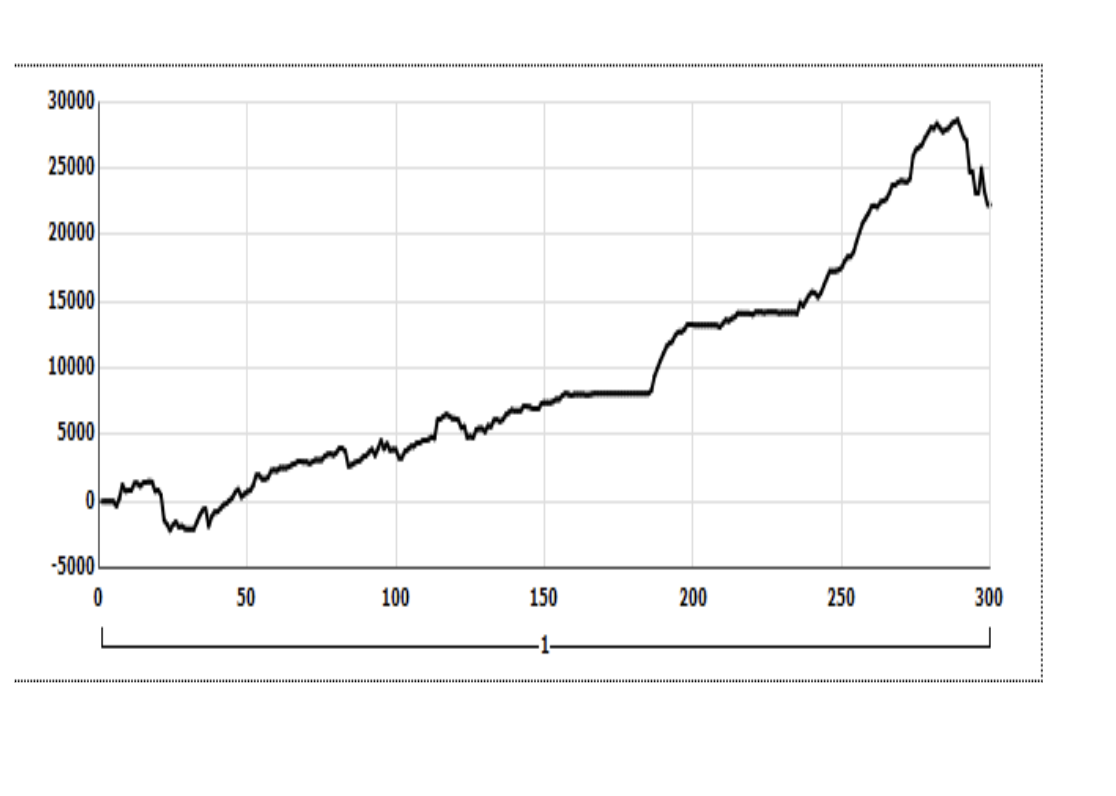
\includegraphics[width=0.7\textwidth]{algo2e_pnl.png}
\caption{P\&L over the second final ALGO2e simulation.}
\label{fig:algo2e_pnl}
\end{figure}

\subsubsection*{Size strategy}

Each stock has a base position size: 10{,}000 shares for RY, 9{,}000 for CNR and 5{,}000 for AC. Together these fit inside the shared limit. Individual orders are at most 5{,}000 shares, as required by the case, and sizes are rounded down to lots of 100.\\

\noindent For momentum positions the size shrinks when the stock is more volatile than usual,
\begin{equation}
N_i = N_i^{\text{base}} \cdot \min\!\left(1,\; \frac{\sigma_i^{\text{ref}}}{\sigma_i}\right),
\end{equation}
where $\sigma_i$ is the current volatility and $\sigma_i^{\text{ref}}$ the stock's normal one-tick volatility. If volatility doubles, the position halves, so the dollar risk per tick stays roughly the same. The size never grows above the base.\\

\noindent For mean-reversion positions the size is not reduced, because a larger swing means a larger profit when the price comes back. Their risk is controlled by two exits instead:
\begin{itemize}
  \item a \textbf{stop-loss}: if the price moves against the position by more than $\max(5\text{c},\, 2.5\,\sigma)$ from the entry price, the position is closed at market and the stock sits out for 10 ticks;
  \item a \textbf{trend guard}: if the move over the last 10 ticks is more than 2.5 times the standard deviation of the stock's recent 10-tick moves (and at least 6 cents), the stock is no longer treated as mean reverting. The position is closed at market and the stock sits out for 10 ticks.
\end{itemize}
Positions only flip through flat: the old position is closed first, and the new one is opened on the next pass.

\subsubsection*{The Python script and how to use it}

The script is \texttt{rit\_algo2e.py} (full listing in the appendix). It needs Python 3.8 or later and the \texttt{requests} package, which is included in Anaconda.
\begin{enumerate}
  \item Start the RIT client, log in to the case and check that the API icon is green. The API port and key are shown in the client's API dialog. The defaults in the script are port 49120 and the key used on our machine; pass \texttt{-{}-port} and \texttt{-{}-key} if they differ.
  \item Check the connection before the case starts. This sends no orders, and prints the case, the three stocks with their fees and rebates, and the position limits:
  \begin{verbatim}
python rit_algo2e.py --check
  \end{verbatim}
  \item Start the algorithm before the case begins:
  \begin{verbatim}
python rit_algo2e.py --keep-running
  \end{verbatim}
  It waits until the case is active, loads recent price history, trades all three stocks, and with \texttt{-{}-keep-running} waits for the next run after each case ends. \texttt{Ctrl+C} stops it and cancels all open orders.
  \item Every five seconds it prints a status line with the NLV, the gross position, and for each stock the regime, the measured $\hat\rho$, the position and target, and the best bid and ask. The same information is written to \texttt{algo2e\_v2\_log.csv}.
\end{enumerate}

\noindent The main options are:

\begin{table}[H]
\centering
\begin{tabular}{ll}
\toprule
Option & Effect \\
\midrule
\texttt{-{}-check} & connection and settings check, no trading \\
\texttt{-{}-paper} & compute targets but send no orders \\
\texttt{-{}-keep-running} & wait for the next run after a case ends \\
\texttt{-{}-size RY=10000 CNR=9000} & base position size per stock \\
\texttt{-{}-size-mult 1.2} & scale every stock's size \\
\texttt{-{}-mode AC=OFF} & force a regime for a stock (MOM, MR or OFF) \\
\texttt{-{}-no-adaptive} & use the default regimes only \\
\texttt{-{}-no-vol-scale} & fixed thresholds and sizes in cents and shares \\
\texttt{-{}-no-mr-stop}, \texttt{-{}-no-mr-trend-guard} & switch off the mean-reversion exits \\
\texttt{-{}-flatten-end} & close all positions in the last two ticks \\
\texttt{-{}-max-reads}, \texttt{-{}-max-writes} & API calls per second (default 180 and 80) \\
\texttt{-{}-interval} & seconds between loops (default 0.08) \\
\bottomrule
\end{tabular}
\caption{Command-line options of \texttt{rit\_algo2e.py}.}
\label{tab:algo2e_options}
\end{table}

\noindent Each loop of the algorithm does the following:
\begin{enumerate}
  \item reads the case status and tick, and waits if the case is not active;
  \item reads our open orders, positions and the order book of each stock, and separates our own orders from those of other traders;
  \item updates each stock's price history, volatility $\sigma$, autocorrelation $\hat\rho$ and EMA, and picks its regime;
  \item sets a target position for each stock from the rules in Table~\ref{tab:algo2e_rules}, including the trailing stop, stop-loss and trend guard;
  \item cancels any resting orders that would let the worst-case position exceed the limit;
  \item moves each stock toward its target, reducing positions first: marketable limit orders for momentum and for forced exits, a single passive limit order at the best price for mean reversion.
\end{enumerate}

\subsection{What was our P\&L?}

Our P\&L in the second final simulation was \textbf{\$22{,}240.40}, which placed us \textbf{second}. The algorithm also finished in the top two in every test simulation.\\

\noindent The first final simulation is not a meaningful comparison. One group pushed RY from about \$100 to \$401 by repeatedly buying at the ask without ever selling, and the end-of-case close-out at the last trade price of \$434.69 turned a 13.1 million share position into about \$4.29 billion of P\&L. That number reflects the zero market impact of the RIT close-out, not trading skill, and the same rally worked directly against our mean-reversion strategy on RY.





\end{document}